
\section{Time Graph of Variables with Different Scales  \label{sec:differentVariables}}
\label{sec:org7e324c2}
There is a variety of scientific research interested in the
relationship among several meteorological variables. A suitable
approach is to display the time evolution of all of them using a
panel for each of the variables. The superposition of variables
with different characteristics is not very useful (unless their
values were previously rescaled), so this option is postponed for
Section \ref{SEC:sameScale}.

For this example we will use the 8 years of daily data from the
SIAR meteorological station located at Aranjuez (Madrid).  This
multivariate time series can be displayed with the \texttt{xyplot} method of
\texttt{lattice} for \texttt{zoo} objects with a panel for each variable (Figure
\ref{fig:aranjuezNaive}).

\lstset{language=r,label= ,caption= ,captionpos=b,numbers=none}
\begin{lstlisting}
library(zoo)
load('data/aranjuez.RData')
\end{lstlisting}

\lstset{language=r,label= ,caption= ,captionpos=b,numbers=none}
\begin{lstlisting}
## The layout argument arranges panels in rows
xyplot(aranjuez, layout = c(1, ncol(aranjuez)))
\end{lstlisting}


\begin{figure}[htbp]
\centering
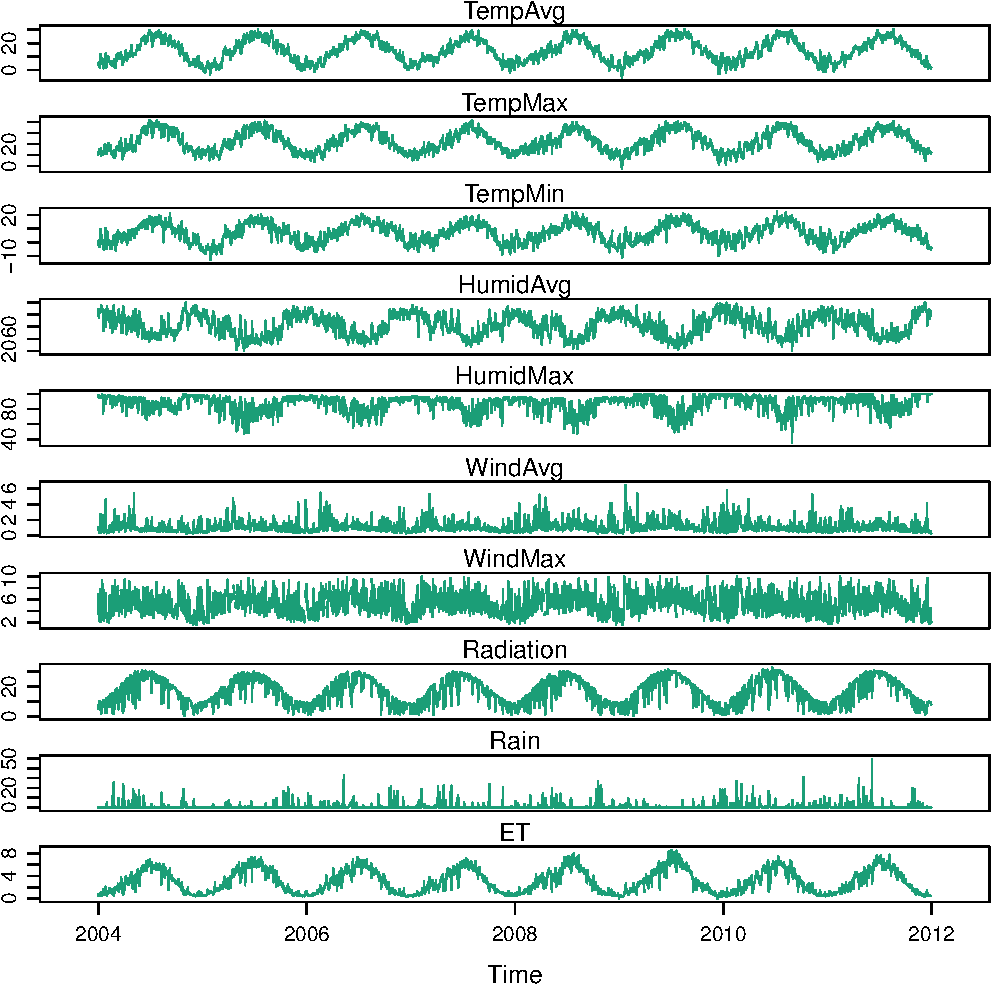
\includegraphics[width=.9\linewidth]{figs/aranjuez.pdf}
\caption{Time plot of the collection of meteorological time series of the Aranjuez station (\texttt{lattice} version). \label{fig:aranjuezNaive}}
\end{figure}

The package \texttt{ggplot2} provides the generic method \texttt{autoplot} to
automate the display of certain classes with a simple command. The
package \texttt{zoo} provides an \texttt{autoplot} method for the \texttt{zoo} class with a
result similar to that obtained with \texttt{xyplot} (Figure \ref{fig:aranjuezNaiveGG})

\lstset{language=r,label= ,caption= ,captionpos=b,numbers=none}
\begin{lstlisting}
autoplot(aranjuez) + facet_free()
\end{lstlisting}

\begin{figure}[htbp]
\centering
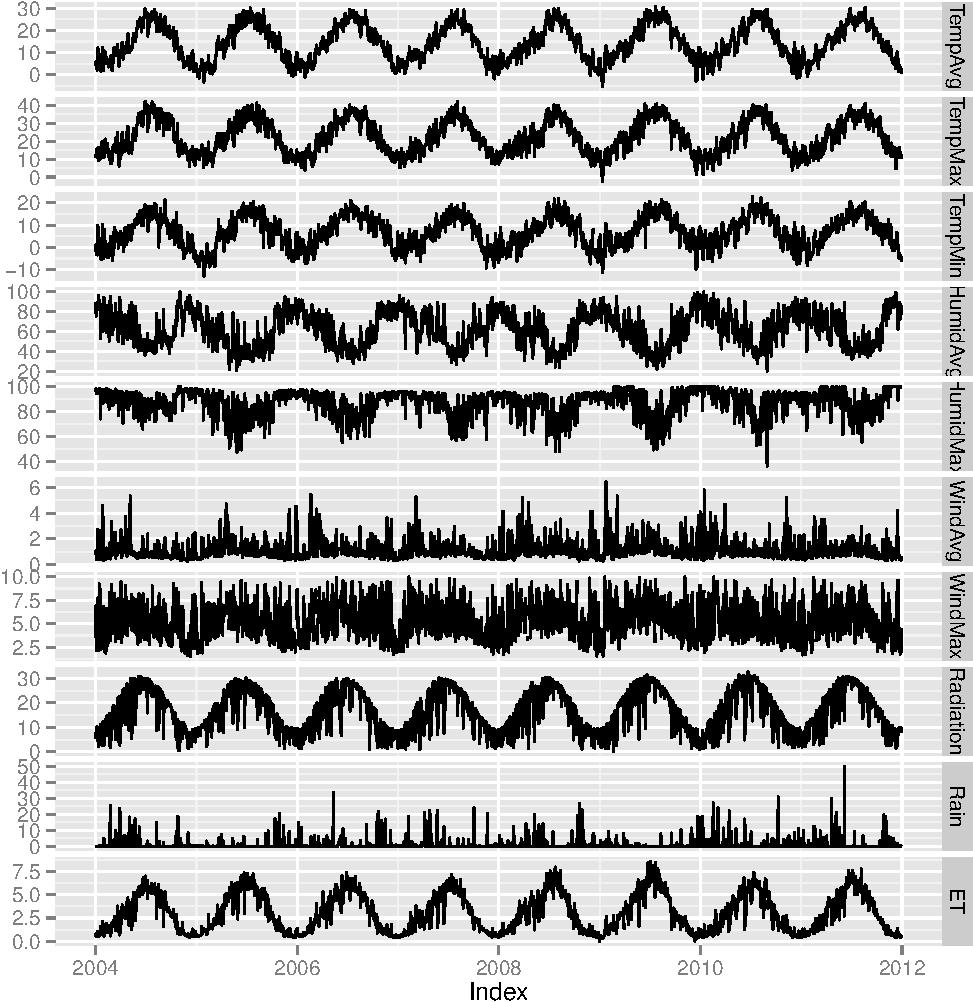
\includegraphics[width=.9\linewidth]{figs/aranjuezGG.pdf}
\caption{Time plot of the collection of meteorological time series of the Aranjuez station (\texttt{ggplot2} version). \label{fig:aranjuezNaiveGG}}
\end{figure}


\subsection{\floweroneleft Annotations to Enhance the Time Graph}
\label{sec:orgf6727db}

These first attempts can be improved with a custom panel function
that generates the content of each panel using the information
processed by \texttt{xyplot}, or overlaying additional layers with
\texttt{autoplot}.  One of the main enhancements is to highlight certain time
regions that fulfill certain conditions. The package \texttt{latticeExtra}
provides a nice solution for \texttt{xyplot} with \texttt{panel.xblocks}. The result
is displayed in Figure \ref{fig:aranjuezEnhanced}:

\begin{itemize}
\item The label of each time series is displayed with text inside each
panel instead of using the strips mechanism. The \texttt{panel.text}
prints the name of each variable with the aid of \texttt{panel.number}.
\item The alternating of years is displayed with blocks of gray and
white color using the \texttt{panel.xblocks} function from
\texttt{latticeExtra}. The year is extracted (as character) from the
time index of the \texttt{zoo} object with \texttt{format.POSIXlt}.
\item Those values below the mean of each variable are highlighted
with short red color blocks at the bottom of each panel, again
with the \texttt{panel.xblocks} function.
\item The maxima and minima are highlighted with small blue triangles.
\end{itemize}

Because the functions included in the panel function are executed
consecutively, their order determines the superposition of graphical
layers.

\index{Panel function}
\index{panel.xblocks@\texttt{panel.xblocks}}
\index{panel.text@\texttt{panel.text}}
\index{panel.number@\texttt{panel.number}}
\index{panel.points@\texttt{panel.points}}


\lstset{language=r,label= ,caption= ,captionpos=b,numbers=none}
\begin{lstlisting}
library(grid)
library(latticeExtra)
  
## Auxiliary function to extract the year value of a POSIXct time
## index
Year <- function(x)format(x, "%Y")
  
xyplot(aranjuez, layout = c(1, ncol(aranjuez)), strip = FALSE,
       scales = list(y = list(cex = 0.6, rot = 0)),
       panel = function(x, y, ...){
           ## Alternation of years
           panel.xblocks(x, Year,
                         col = c("lightgray", "white"),
                         border = "darkgray")
           ## Values under the average highlighted with red regions
           panel.xblocks(x, y<mean(y, na.rm = TRUE),
                         col = "indianred1",
                         height = unit(0.1, 'npc'))
           ## Time series
           panel.lines(x, y, col = 'royalblue4', lwd = 0.5, ...)
           ## Label of each time series
           panel.text(x[1], min(y, na.rm = TRUE),
                      names(aranjuez)[panel.number()],
                      cex = 0.6, adj = c(0, 0), srt = 90, ...)
           ## Triangles to point the maxima and minima 
           idxMax <- which.max(y)
           panel.points(x[idxMax], y[idxMax],
                        col = 'black', fill = 'lightblue', pch = 24)
           idxMin <- which.min(y)
           panel.points(x[idxMin], y[idxMin],
                        col = 'black', fill = 'lightblue', pch = 25)
       })
\end{lstlisting}

\begin{figure}[htbp]
\centering
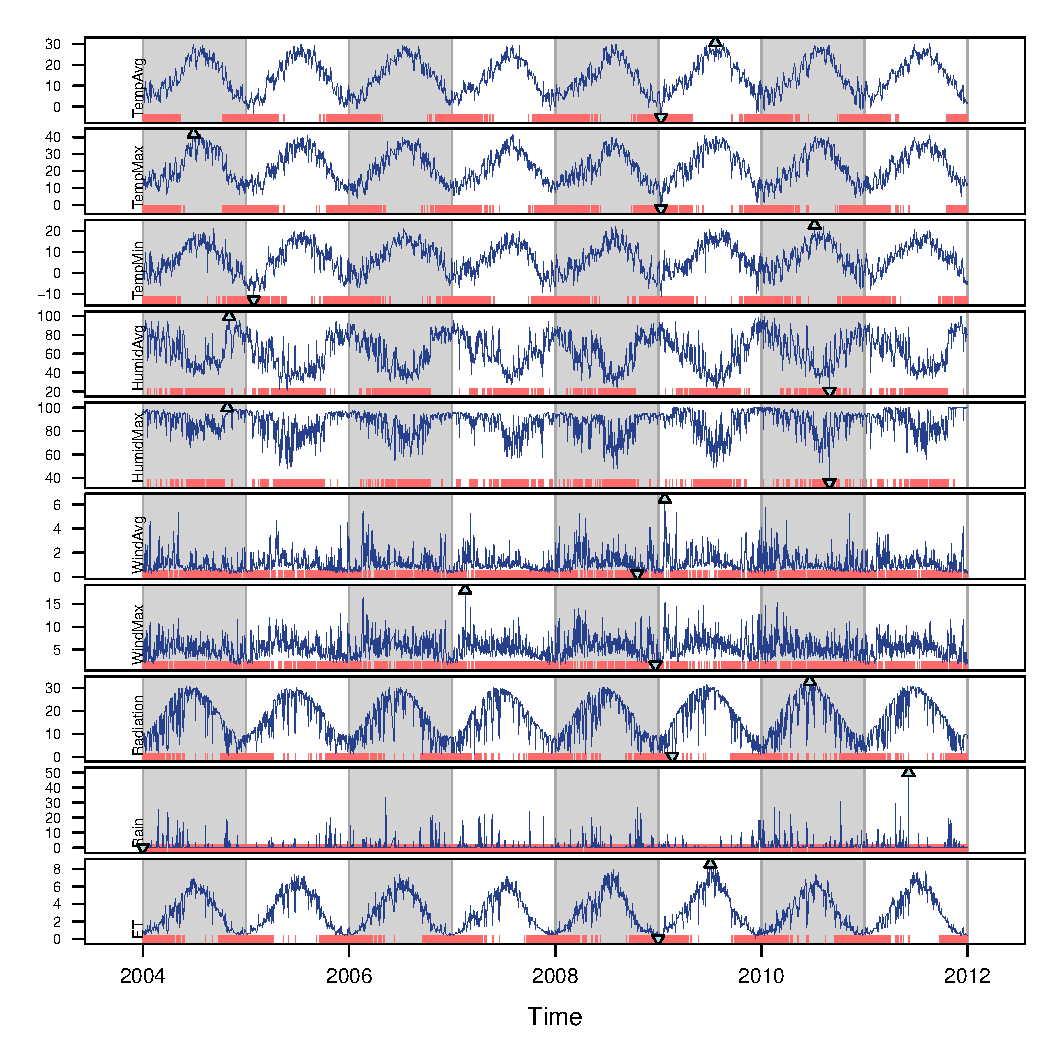
\includegraphics[width=.9\linewidth]{figs/aranjuezXblocks.pdf}
\caption{Enhanced time plot of the collection of meteorological time series of the Aranjuez station. \label{fig:aranjuezEnhanced}}
\end{figure}

There is no equivalent \texttt{panel.xblocks} function that can be used with
\texttt{ggplot2}. Therefore, the \texttt{ggplot2} version must explicitly compute
the corresponding bands (years and regions below the average values):

\begin{itemize}
\item The first step in working with \texttt{ggplot} is to transform the \texttt{zoo}
object into a \texttt{data.frame} in long format. \texttt{fortify} returns a
\texttt{data.frame} with three columns: the time \texttt{Index}, a factor
indicating the \texttt{Series}, and the corresponding \texttt{Value}.
\end{itemize}

\index{fortify@\texttt{fortify}}
\index{melt\texttt{melt}}

\lstset{language=r,label= ,caption= ,captionpos=b,numbers=none}
\begin{lstlisting}
timeIdx <- index(aranjuez)
  
aranjuezLong <- fortify(aranjuez, melt = TRUE)

summary(aranjuezLong)
\end{lstlisting}

\begin{verbatim}
    Index                 Series          Value       
Min.   :2004-01-01   TempAvg : 2898   Min.   :-12.98  
1st Qu.:2005-12-29   TempMax : 2898   1st Qu.:  1.99  
Median :2008-01-09   TempMin : 2898   Median :  8.52  
Mean   :2008-01-03   HumidAvg: 2898   Mean   : 22.09  
3rd Qu.:2010-01-03   HumidMax: 2898   3rd Qu.: 27.71  
Max.   :2011-12-31   WindAvg : 2898   Max.   :100.00  
                     (Other) :11592   NA's   :152
\end{verbatim}

\begin{itemize}
\item The bands of values below the average can be easily extracted with
\texttt{scale} because these regions are negative when the \texttt{data.frame} is
centered.
\end{itemize}

\index{fortify@\texttt{fortify}}
\index{melt\texttt{melt}}

\lstset{language=r,label= ,caption= ,captionpos=b,numbers=none}
\begin{lstlisting}
## Values below mean are negative after being centered
scaled <- fortify(scale(aranjuez, scale = FALSE), melt = TRUE)
## The 'scaled' column is the result of the centering.
## The new 'Value' column store the original values.
scaled <- transform(scaled, scaled = Value, Value = long$Value)
underIdx <- which(scaled$scaled <= 0)
## 'under' is the subset of values below the average
under <- scaled[underIdx,]
\end{lstlisting}

\begin{itemize}
\item The years bands are defined with the function \texttt{endpoints} from the
\texttt{xts} package:
\end{itemize}

\index{Package!xts@\texttt{xts}}

\lstset{language=r,label= ,caption= ,captionpos=b,numbers=none}
\begin{lstlisting}
library(xts)
ep <- endpoints(timeIdx, on = 'years')
ep <- ep[-1]
N <- length(ep)
## 'tsp' is start and 'tep' is the end of each band. One of each two
## years are selected.
tep <- timeIdx[ep[seq(1, N, 2)] + 1]
tsp <- timeIdx[ep[seq(2, N, 2)]]
\end{lstlisting}
\begin{itemize}
\item The minima and maxima points of each variable are extracted with
\texttt{apply}:
\end{itemize}
\lstset{language=r,label= ,caption= ,captionpos=b,numbers=none}
\begin{lstlisting}
minIdx <- timeIdx[apply(aranjuez, 2, which.min)]
minVals <- apply(aranjuez, 2, min, na.rm = TRUE)
mins <- data.frame(Index = minIdx,
                   Value = minVals,
                   Series = names(aranjuez))

maxIdx <- timeIdx[apply(aranjuez, 2, which.max)]
maxVals <- apply(aranjuez, 2, max, na.rm = TRUE)
maxs <- data.frame(Index = maxIdx,
                   Value = maxVals,
                   Series = names(aranjuez))
\end{lstlisting}

\begin{itemize}
\item With \texttt{ggplot} we define the canvas, and the layers of information are
added successively:
\end{itemize}
\lstset{language=r,label= ,caption= ,captionpos=b,numbers=none}
\begin{lstlisting}
ggplot(data = aranjuezLong, aes(Index, Value)) +
    ## Time series of each variable
    geom_line(colour = "royalblue4", lwd = 0.5) +
    ## Year bands
    annotate('rect',
             xmin = tsp, xmax = tep,
             ymin = -Inf, ymax = Inf,
              alpha = 0.4) + 
    ## Values below average
    geom_rug(data = under,
             sides = 'b', col = 'indianred1') +
    ## Minima
    geom_point(data = mins, pch = 25) +
    ## Maxima
    geom_point(data = maxs, pch = 24) +
    ## Axis labels and theme definition
    labs(x = 'Time', y = NULL) +
    theme_bw() +
    ## Each series is displayed in a different panel with an
    ## independent y scale
    facet_free()
\end{lstlisting}

Some messages from Figure \ref{fig:aranjuezEnhanced}:
\begin{itemize}
\item The radiation, temperature, and evotranspiration are
quasi-periodic and are almost synchronized between them. Their
local maxima appear in the summer and the local minima in the
winter. Obviously, the summer values are higher than the
average.
\item The average humidity varies in oposition to the temperature and
radiation cycle, with local maxima located during winter.
\item The average and maximum wind speed, and rainfall vary in a more
erratic way and do not show the evident periodic behavior of
the radiation and temperature.
\item The rainfall is different from year to year. The remaining variables
do not show variations between years.
\item The fluctuations of solar radiation are more apparent than
the temperature fluctuations. There is hardly any day with
temperatures below the average value during summer, while it is
not difficult to find days with radiation below the average
during this season.
\end{itemize}

\section{Time Series of Variables with the Same Scale \label{SEC:sameScale}}
\label{sec:orgc95635e}
As an example of time series of variables with the same scale, we will
use measurements of solar radiation from different meteorological
stations.

The first attempt to display this multivariate time series makes use
of the \texttt{xyplot.zoo} method. The objective of this graphic is to
display the behavior of the collection as a whole: the series are
superposed in the same panel (\texttt{superpose=TRUE}) without legend
(\texttt{auto.key=TRUE}), using thin lines and partial
transparency\footnote{A similar result can be obtained with \texttt{autoplot} using \texttt{facets=NULL}.}. Transparency softens overplotting problems and reveals
density clusters because regions with more overlapping lines are
darker. Figure \ref{fig:navarraNaive} displays the variations
around the time average (\texttt{avRad}).

\lstset{language=r,label= ,caption= ,captionpos=b,numbers=none}
\begin{lstlisting}
load('data/navarra.RData')
\end{lstlisting}

\index{zoo@\texttt{zoo}}
\index{xyplot.zoo@\texttt{xyplot.zoo}}

\lstset{language=r,label= ,caption= ,captionpos=b,numbers=none}
\begin{lstlisting}
avRad <- zoo(rowMeans(navarra, na.rm = 1), index(navarra))
pNavarra <- xyplot(navarra - avRad,
                   superpose = TRUE, auto.key = FALSE,
                   lwd = 0.5, alpha = 0.3, col = 'midnightblue') 
pNavarra
\end{lstlisting}

\begin{figure}[htbp]
\centering
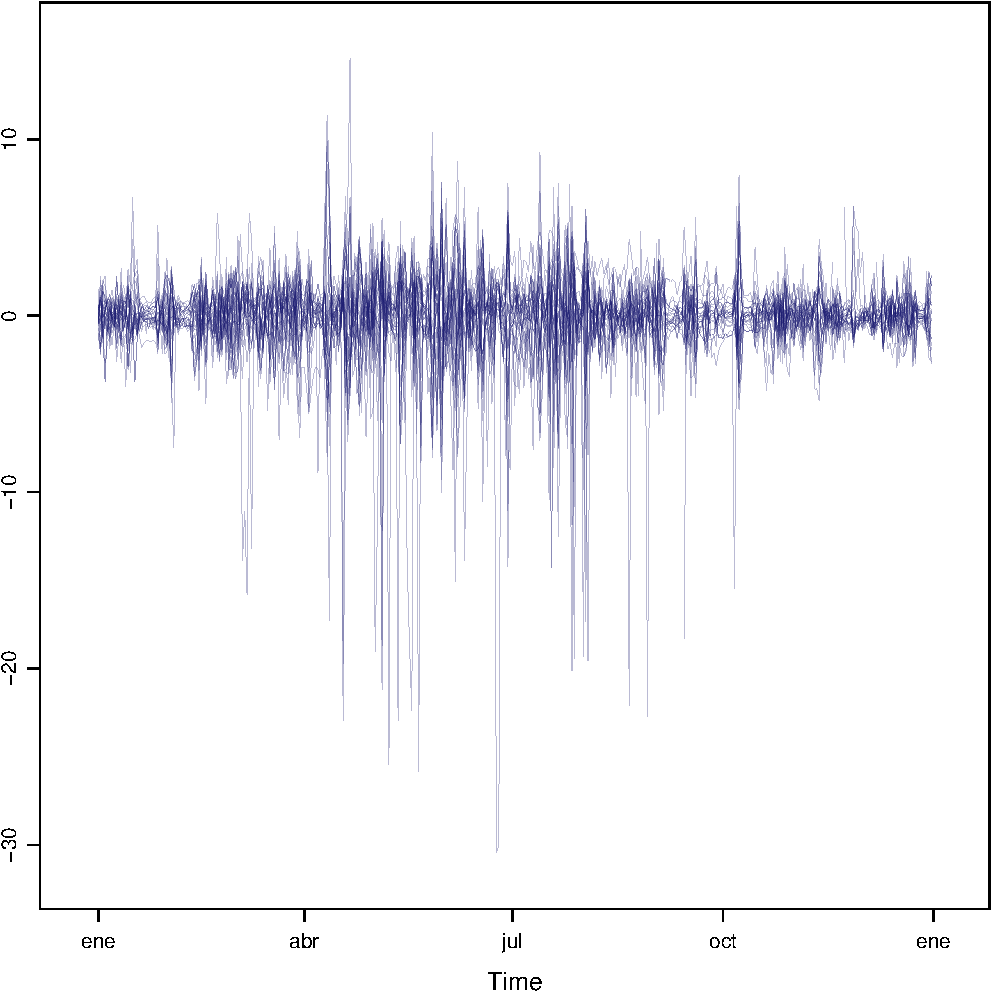
\includegraphics[width=.9\linewidth]{figs/navarra.pdf}
\caption{Time plot of the variations around time average of solar radiation measurements from the meteorological stations of Navarra. \label{fig:navarraNaive}}
\end{figure}

This result can be improved with different methods: the cut-and-stack
method, and the horizon graph with \texttt{horizonplot}.

\subsection{Aspect Ratio and Rate of Change}
\label{sec:org6e9d855}
When a graphic is intended to inform about the rate of change,
special attention must be paid to the aspect ratio of the graph,
defined as the ratio of the height to the width of the graphical
window. Cleveland analyzed the importance of the aspect ratio for
judging rate of change. He concluded that we visually decode the
information about the relative local rate of change of one
variable with another by comparing the orientations of the local
line segments that compose the polylines. The recommendation is to
choose the aspect ratio so that the absolute values of the
orientations of the segments are centered on \(\SI{45}{\degree}\) (banking
to \(\SI{45}{\degree}\)). 

The problem with banking to \(\SI{45}{\degree}\) is that the resulting
aspect ratio is frequently too small. A suitable solution to
minimize wasted space is the cut-and-stack method. The \texttt{xyplot.ts}
method implement this solution with the combination of the
arguments \texttt{aspect} and \texttt{cut}. The version of Figure
\ref{fig:navarraNaive} using banking to \(\SI{45}{\degree}\) and the
cut-and-stack method is produced with
\lstset{language=r,label= ,caption= ,captionpos=b,numbers=none}
\begin{lstlisting}
xyplot(navarra - avRad,
       aspect = 'xy', cut = list(n = 3, overlap = 0.1),
       strip = FALSE,
       superpose = TRUE, auto.key = FALSE,
       lwd = 0.5, alpha = 0.3, col = 'midnightblue')
\end{lstlisting}

\begin{figure}[htbp]
\centering
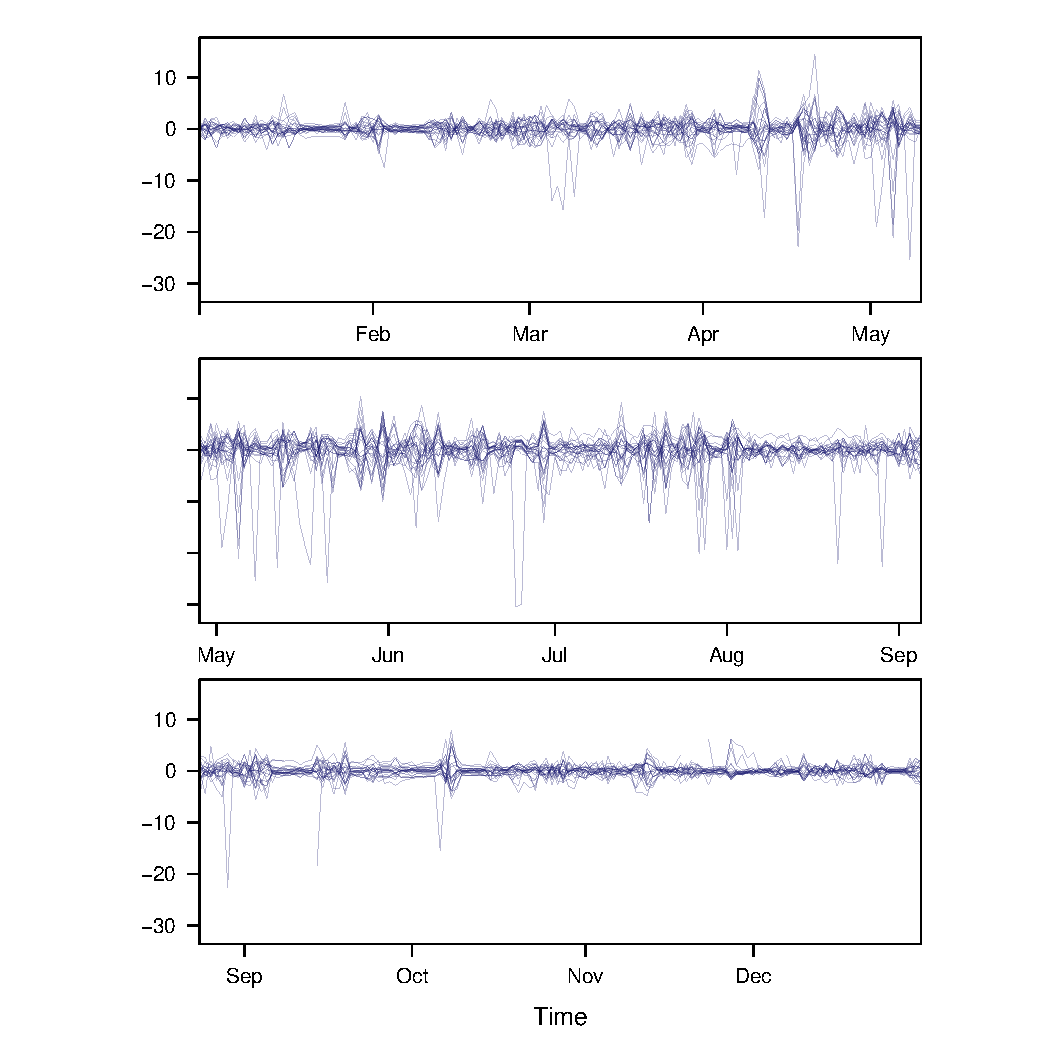
\includegraphics[width=.9\linewidth]{figs/navarraBanking.pdf}
\caption{Cut-and-stack plot with banking to \(\SI{45}{\degree}\). \label{fig:navarraBanking}}
\end{figure}

\subsection{The Horizon Graph \label{sec:horizonplot}}
\label{sec:orge7e24cf}
\index{Horizon graph}
The horizon graph is useful in examining how a large number of series
changes over time, and does so in a way that allows both comparisons
between the individual time series and and independent analysis of
each series. Moreover, extraordinary behaviors and predominant
patterns are easily distinguished \cite{Heer.Kong.ea2009,Few2008}.

This graph displays several stacked series collapsing the y-axis
to free vertical space:
\begin{itemize}
\item Positive and negative values share the same vertical
space. Negative values are inverted and placed above the
reference line. Sign is encoded using different hues (positive
values in blue and negative values in red).
\item Differences in magnitude are displayed as differences in color
intensity (darker colors for greater differences).
\item The color bands share the same baseline and are superposed, with
darker bands in front of the ligther ones.
\end{itemize}

Because the panels share the same design structure, once this
technique is understood, it is easy to establish comparisons or spot
extraordinary events.  This method is what Tufte described as small
multiples\#+INDEX: Small multiples\} \cite{Tufte1990}.

Figure \ref{fig:navarraHorizonplot} displays the variations of
solar radiation around the time average with an horizon graph
using a row for each time series.

\index{Packages!latticeExtra@\texttt{latticeExtra}}
\index{horizonplot@\texttt{horizonplot}}

\lstset{language=r,label= ,caption= ,captionpos=b,numbers=none}
\begin{lstlisting}
library(latticeExtra)
  
horizonplot(navarra-avRad,
            layout = c(1, ncol(navarra)),
            origin = 0, colorkey = TRUE)
\end{lstlisting}

\begin{figure}[htbp]
\centering
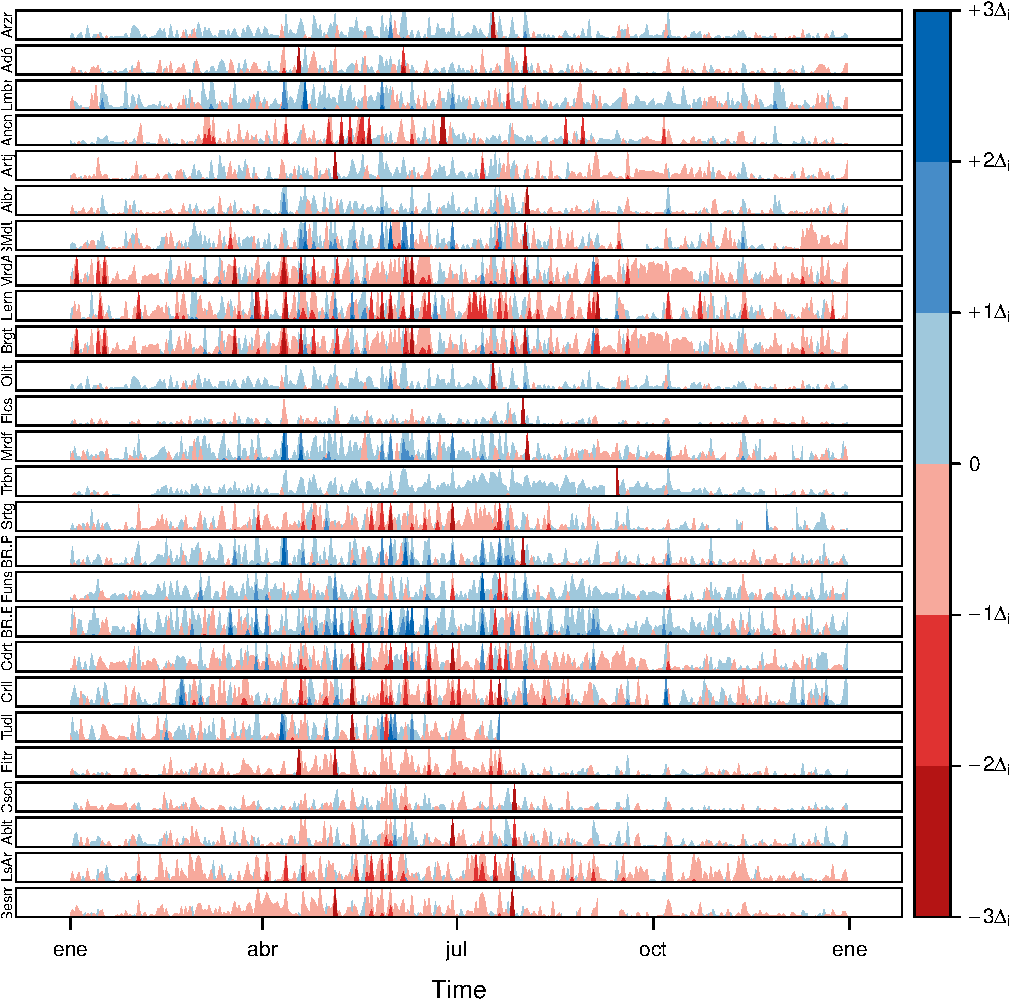
\includegraphics[width=.9\linewidth]{figs/navarraHorizonplot.pdf}
\caption{Horizon plot of variations around time average of solar radiation measurements from the meteorological stations of Navarra. \label{fig:navarraHorizonplot}}
\end{figure}

Figure \ref{fig:navarraHorizonplot} allows several questions to be
answered:
\begin{itemize}
\item Which stations consistently measure above and below the average?
\item Which stations resemble more closely the average time series?
\item Which stations show erratic and uniform behavior?
\item In each of the stations, is there any day with extraordinary measurements?
\item Which part of the year is associated with more intense
absolute fluctuations across the set of stations?
\end{itemize}

\subsection{Time Graph of the Differences between a Time Series and a Reference \label{sec:differences}}
\label{sec:org4ac6204}

The horizon graph is also useful in revealing the differences between
a univariate time series and another reference. For example, we
might be interested in the departure of the observed temperature
from the long-term average, or in other words, the temperature
change over time.

Let's illustrate this approach with the time series of daily
average temperatures measured at the meteorological station of
Aranjuez. The reference is the long-term daily average calculated
with \texttt{ave}.

\lstset{language=r,label= ,caption= ,captionpos=b,numbers=none}
\begin{lstlisting}
Ta <- aranjuez$TempAvg
timeIndex <- index(aranjuez)
longTa <- ave(Ta, format(timeIndex, '%j'))
diffTa <- (Ta - longTa)
\end{lstlisting}


The temperature time series, the long-term average and the
differences between them can be displayed with the \texttt{xyplot}
method, now using \texttt{screens} to use a different panel for the
differences time series (Figure \ref{fig:diffTa_xyplot})
\lstset{language=r,label= ,caption= ,captionpos=b,numbers=none}
\begin{lstlisting}
xyplot(cbind(Ta, longTa, diffTa),
       col = c('darkgray', 'red', 'midnightblue'),
       superpose = TRUE, auto.key = list(space = 'right'),
       screens = c(rep('Average Temperature', 2), 'Differences'))
\end{lstlisting}

\begin{figure}[htbp]
\centering
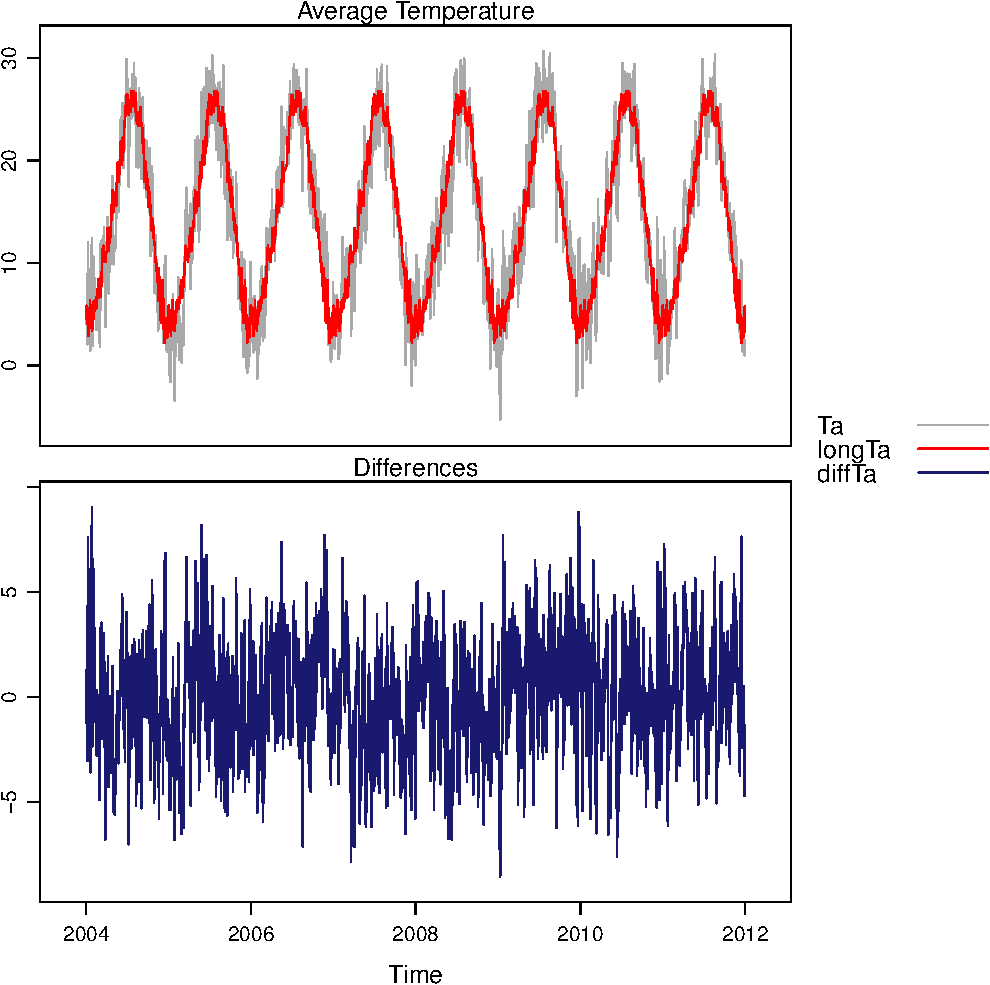
\includegraphics[width=.9\linewidth]{figs/diffTa_xyplot.pdf}
\caption{Daily temperature time series, its long-term average and the differences between them. \label{fig:diffTa_xyplot}}
\end{figure}

The horizon graph is better suited for displaying the differences. The
next code again uses the cut-and-stack method (Figure
\ref{fig:navarraBanking}) to distinguish between years. Figure
\ref{fig:diffTa_horizon} shows that 2004 started clearly above the
average while 2005 and 2009 did the contrary. Year 2007 was frequently
below the long-term average but 2011 was more similar to that
reference.
\lstset{language=r,label= ,caption= ,captionpos=b,numbers=none}
\begin{lstlisting}
years <- unique(format(timeIndex, '%Y'))
  
horizonplot(diffTa, cut = list(n = 8, overlap = 0),
            colorkey = TRUE, layout = c(1, 8),
            scales = list(draw = FALSE, y = list(relation = 'same')),
            origin = 0, strip.left = FALSE) +
    layer(grid.text(years[panel.number()], x  =  0, y  =  0.1, 
                    gp = gpar(cex = 0.8),
                    just = "left"))
\end{lstlisting}

\begin{figure}[htbp]
\centering
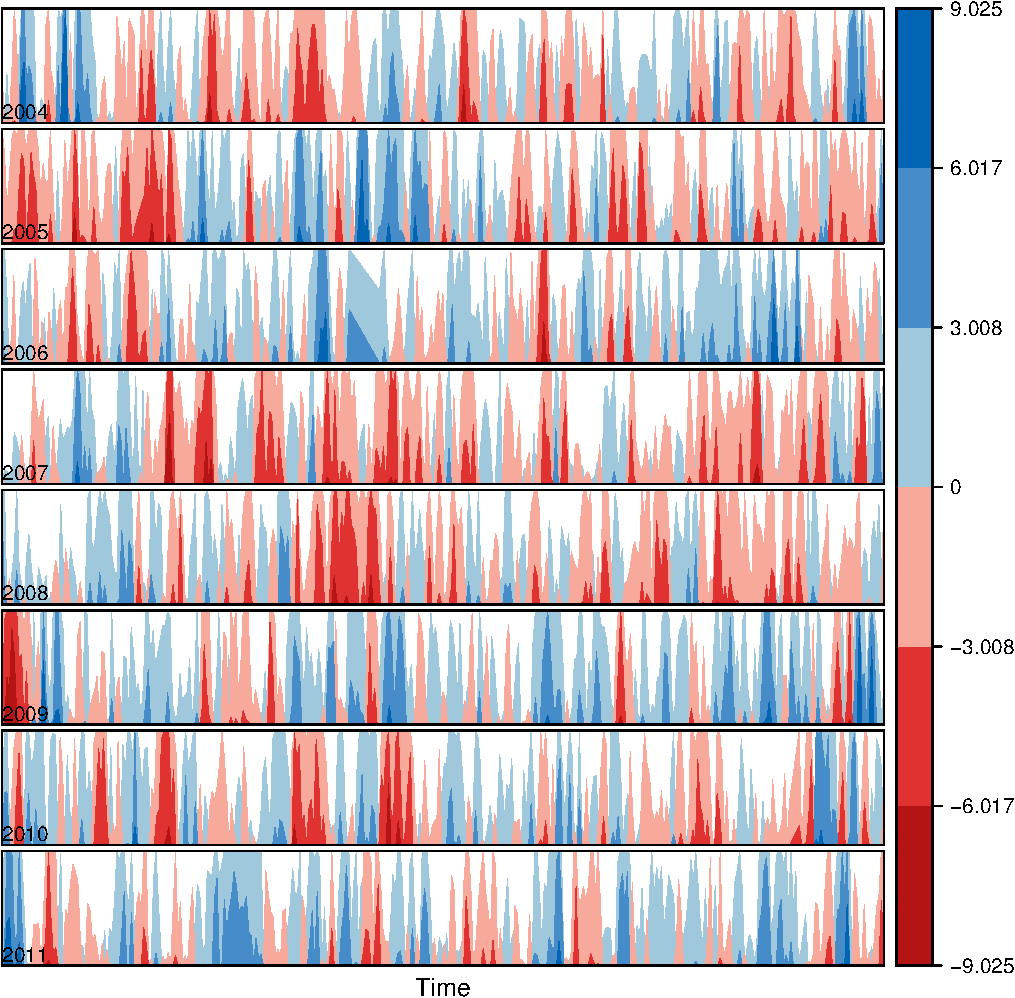
\includegraphics[width=.9\linewidth]{figs/diffTa_horizon.pdf}
\caption{Horizon graph displaying differences between a daily temperature time series and its long-term average. \label{fig:diffTa_horizon}}
\end{figure}

A different approach to display this information is to produce a level
plot displaying the time series using parts of its time index as
independent and conditioning variables\footnote{This approach was inspired by the \texttt{strip} function of the
\texttt{metvurst} package
\url{https://metvurst.wordpress.com/2013/03/04/visualising-large-amounts-of-hourly-environmental-data-2/}.}. The following code
displays the differences with the day of month on the horizontal axis
and the year on the vertical axis, with a different panel for each
month number. Therefore, each cell of Figure \ref{fig:diffTa_level}
corresponds to a certain day of the time series. If you compare this
figure with the horizon plot, you will find the same previous findings
but revealed now in more detail. On the other hand, while the horizon
plot of Figure \ref{fig:diffTa_horizon} clearly displays the yearly
evolution, the combination of variables of the level plot focuses on
the comparison between years in a certain month.

\lstset{language=r,label= ,caption= ,captionpos=b,numbers=none}
\begin{lstlisting}
year <- function(x)as.numeric(format(x, '%Y'))
day <- function(x)as.numeric(format(x, '%d'))
month <- function(x)as.numeric(format(x, '%m'))
\end{lstlisting}

\lstset{language=r,label= ,caption= ,captionpos=b,numbers=none}
\begin{lstlisting}
myTheme <- modifyList(custom.theme(region = brewer.pal(9, 'RdBu')),
                      list(
                          strip.background = list(col = 'gray'),
                          panel.background = list(col = 'gray')))

maxZ <- max(abs(diffTa))

levelplot(diffTa ~ day(timeIndex) * year(timeIndex) | factor(month(timeIndex)),
          at = pretty(c(-maxZ, maxZ), n = 8),
          colorkey = list(height = 0.3),
          layout = c(1, 12), strip = FALSE, strip.left = TRUE,
          xlab = 'Day', ylab = 'Month', 
          par.settings = myTheme)

\end{lstlisting}

\begin{figure}[htbp]
\centering
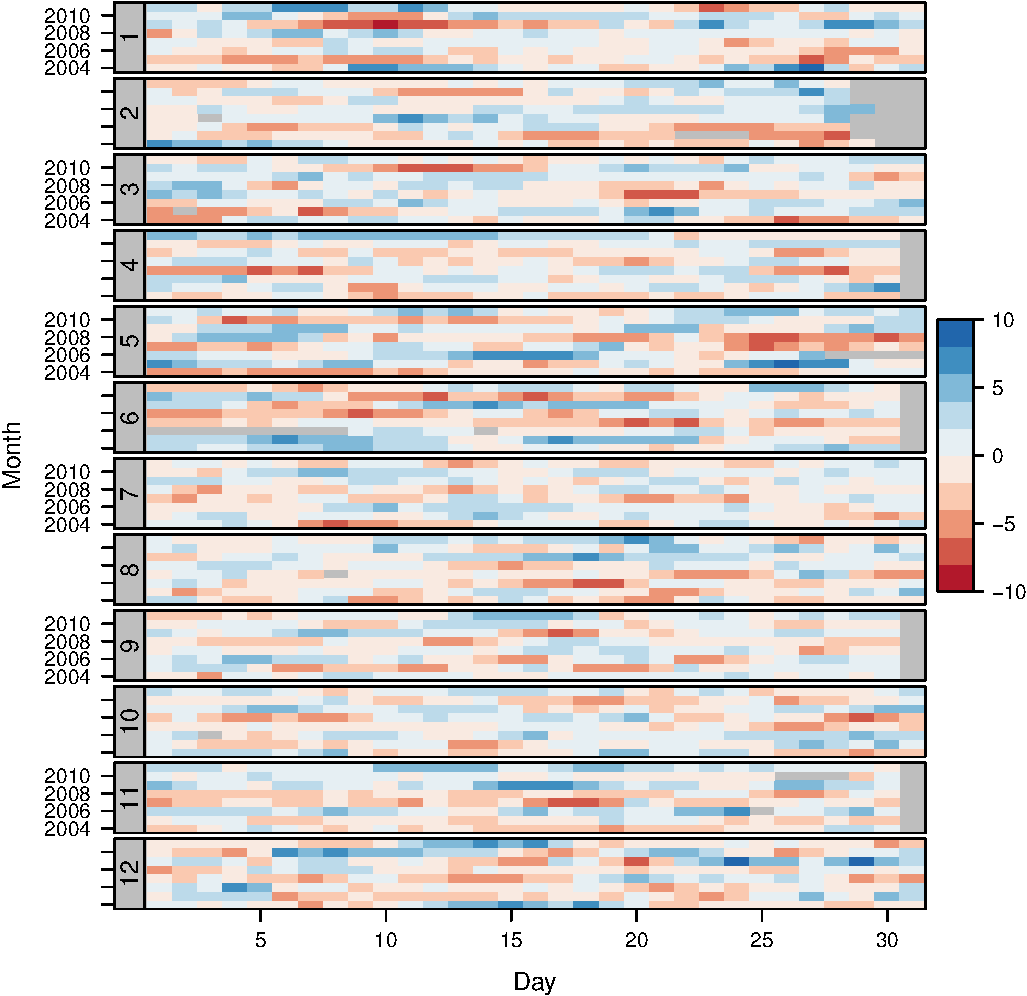
\includegraphics[width=.9\linewidth]{figs/diffTa_levelplot.pdf}
\caption{Level plot of differences between a daily temperature time series and its long-term average. \label{fig:diffTa_level}}
\end{figure}

The \texttt{ggplot} version of the Figure  \ref{fig:diffTa_level} requires a \texttt{data.frame} with the day, year, and month arranged in different columns.
\lstset{language=r,label= ,caption= ,captionpos=b,numbers=none}
\begin{lstlisting}
df <- data.frame(Vals = diffTa,
                 Day = day(timeIndex),
                 Year = year(timeIndex),
                 Month = month(timeIndex))
\end{lstlisting}

The values (\texttt{Vals} column of this \texttt{data.frame}) are displayed as a level plot thanks to the \texttt{geom\_raster} function.
\lstset{language=r,label= ,caption= ,captionpos=b,numbers=none}
\begin{lstlisting}
library(scales) 
## The packages scales is needed for the pretty_breaks function.

ggplot(data = df,
       aes(fill = Vals,
           x = Day,
           y = Year)) +
    facet_wrap(~ Month, ncol = 1, strip.position = 'left') +
    scale_y_continuous(breaks = pretty_breaks()) + 
    scale_fill_distiller(palette = 'RdBu', direction = 1) + 
    geom_raster() +
    theme(panel.grid.major = element_blank(),
          panel.grid.minor = element_blank())
\end{lstlisting}



\section{Stacked Graphs \label{sec:stacked}}
\label{sec:org3093cb5}
If the variables of a multivariate time series can be summed to
produce a meaningful global variable, they may be better displayed
with stacked graphs. For example, the information on unemployment in
the United States provides data of unemployed persons by industry and
class of workers, and can be summed to give a total unemployment time
series.

\lstset{language=r,label= ,caption= ,captionpos=b,numbers=none}
\begin{lstlisting}
load('data/unemployUSA.RData')
\end{lstlisting}

The time series of unemployment can be directly displayed
with the \texttt{xyplot.zoo} method (Figure \ref{fig:unemployUSAxyplot}).

\lstset{language=r,label= ,caption= ,captionpos=b,numbers=none}
\begin{lstlisting}
xyplot(unemployUSA,
       superpose = TRUE,
       par.settings = custom.theme,
       auto.key = list(space = 'right'))
\end{lstlisting}

\begin{figure}[htbp]
\centering
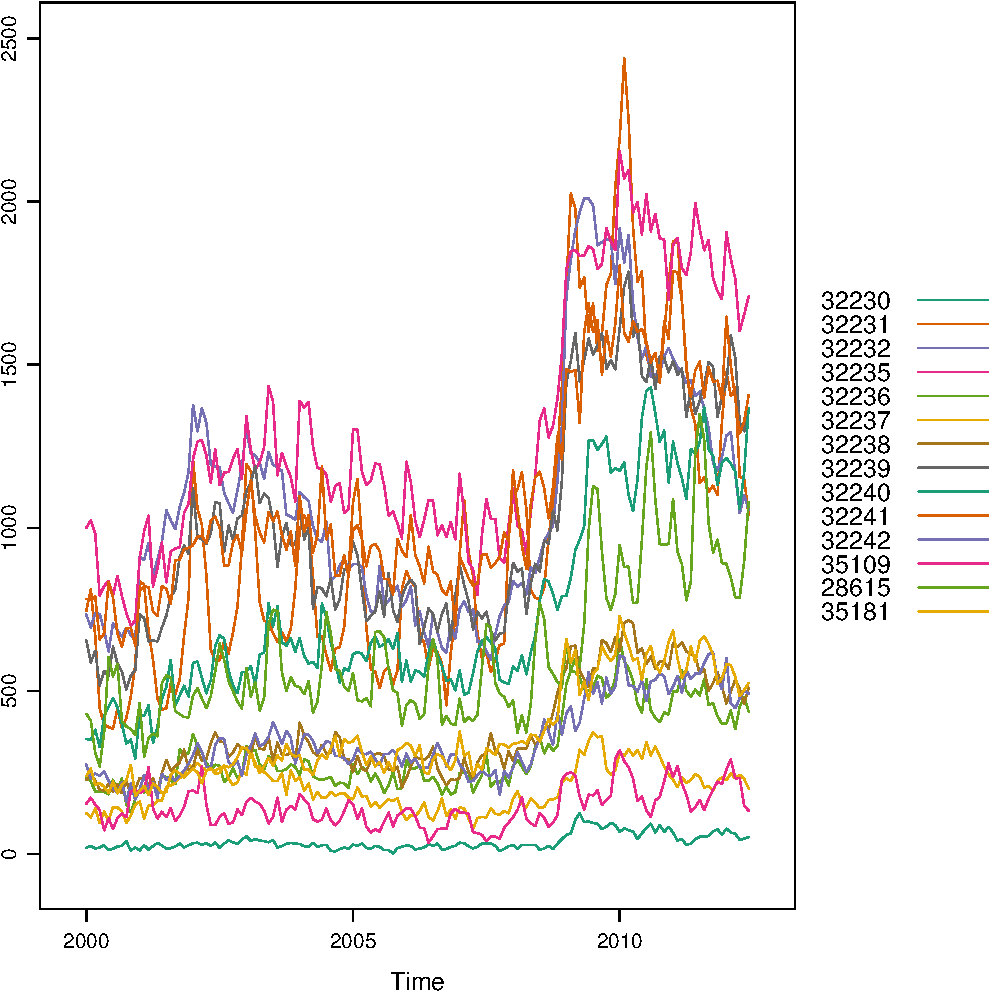
\includegraphics[width=.9\linewidth]{figs/unemployUSAxyplot.pdf}
\caption{Time series of unemployment  with \texttt{xyplot} using the default panel function. \label{fig:unemployUSAxyplot}}
\end{figure}

This graphical output is not very useful: the legend is confusing,
with too many items; the vertical scale is dominated by the largest
series, with several series buried in the lower part of the scale; the
trend, variations and structure of the total and individual
contributions cannot be deduced from this graph.

A suitable improvement is to display the multivariate time series as a
set of stacked colored polygons to follow the macro/micro principle
proposed by Tufte \cite{Tufte1990}: Show a collection of individual
time series and also display their sum. A traditional stacked graph is
easily obtained with \texttt{geom\_area} (Figure \ref{fig:unemployUSAgeomArea}):

\lstset{language=r,label= ,caption= ,captionpos=b,numbers=none}
\begin{lstlisting}
library(scales) ## scale_x_yearmon needs scales::pretty_breaks
autoplot(unemployUSA, facets = NULL, geom = 'area') +
    geom_area(aes(fill = Series)) +
    scale_x_yearmon()  
\end{lstlisting}

\begin{figure}[htbp]
\centering
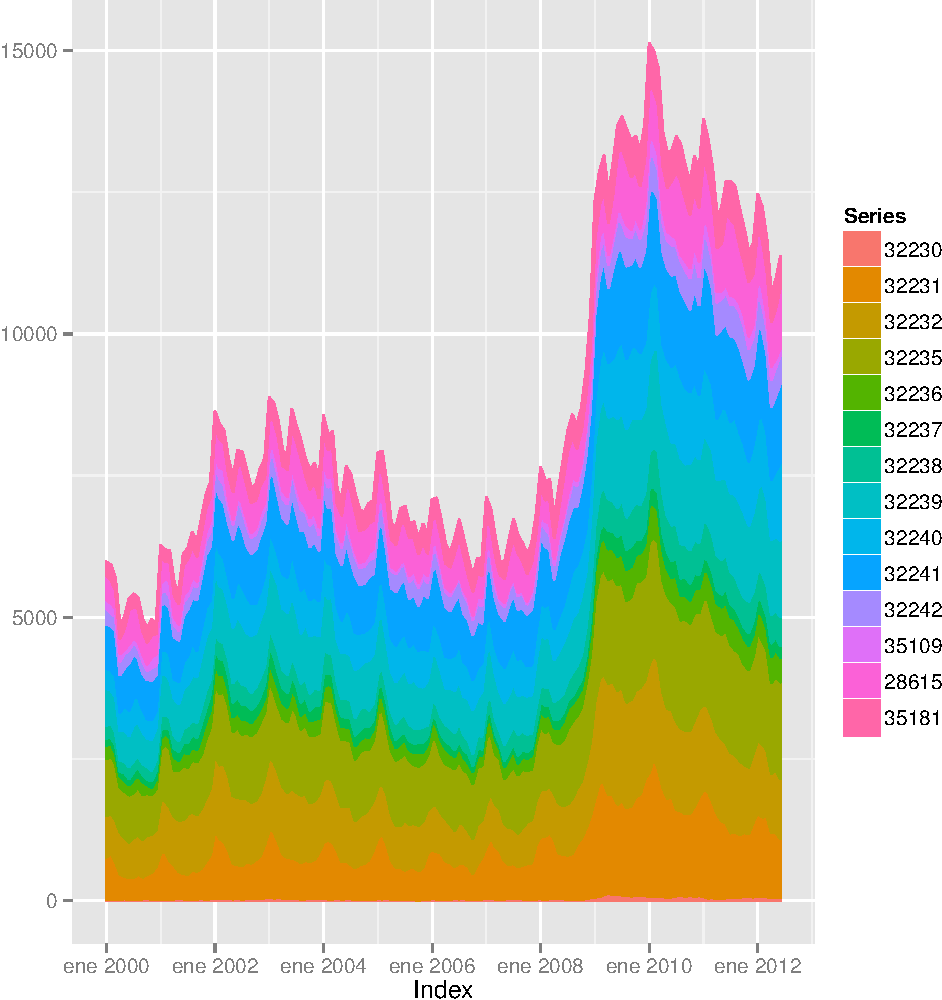
\includegraphics[width=.9\linewidth]{figs/unemployUSAgeomArea.pdf}
\caption{Time series of unemployment with stacked areas using \texttt{geom\_area}. \label{fig:unemployUSAgeomArea}}
\end{figure}

Traditional stacked graphs have their bottom on the x-axis which makes
the overall height at each point easy to estimate. On the other hand,
with this layout, individual layers may be difficult to
distinguish. The \emph{ThemeRiver} \cite{Havre.Hetzler.ea2002} (also named
\emph{streamgraph} in \cite{Byron.Wattenberg2008}) provides an innovative
layout method in which layers are symmetrical around the x-axis at
their center. At a glance, the pattern of the global sum and
individual variables, their contribution to conform the global sum,
and the interrelation between variables can be perceived.

I have defined a panel and prepanel functions\footnote{The code of these panel and prepanel functions is explained
in Section \ref{sec:themeRiverPanel}.} to implement a
ThemeRiver with \texttt{xyplot}. The result is displayed in Figure
\ref{fig:unemployUSAThemeRiver} with a vertical line to indicate
one of main milestones of the financial crisis, whose effect on
the overall unemployment results is clearly evident.
\lstset{language=r,label= ,caption= ,captionpos=b,numbers=none}
\begin{lstlisting}
library(colorspace)
## We will use a qualitative palette from colorspace
nCols <- ncol(unemployUSA)
pal <- rainbow_hcl(nCols, c = 70, l = 75, start = 30, end = 300)
myTheme <- custom.theme(fill = pal, lwd = 0.2)

sep2008 <- as.numeric(as.yearmon('2008-09'))

xyplot(unemployUSA, superpose = TRUE, auto.key = FALSE,
       panel = panel.flow, prepanel = prepanel.flow,
       origin = 'themeRiver', scales = list(y = list(draw = FALSE)),
       par.settings = myTheme) +
    layer(panel.abline(v = sep2008, col = 'gray', lwd = 0.7))
\end{lstlisting}

\begin{figure}[htbp]
\centering
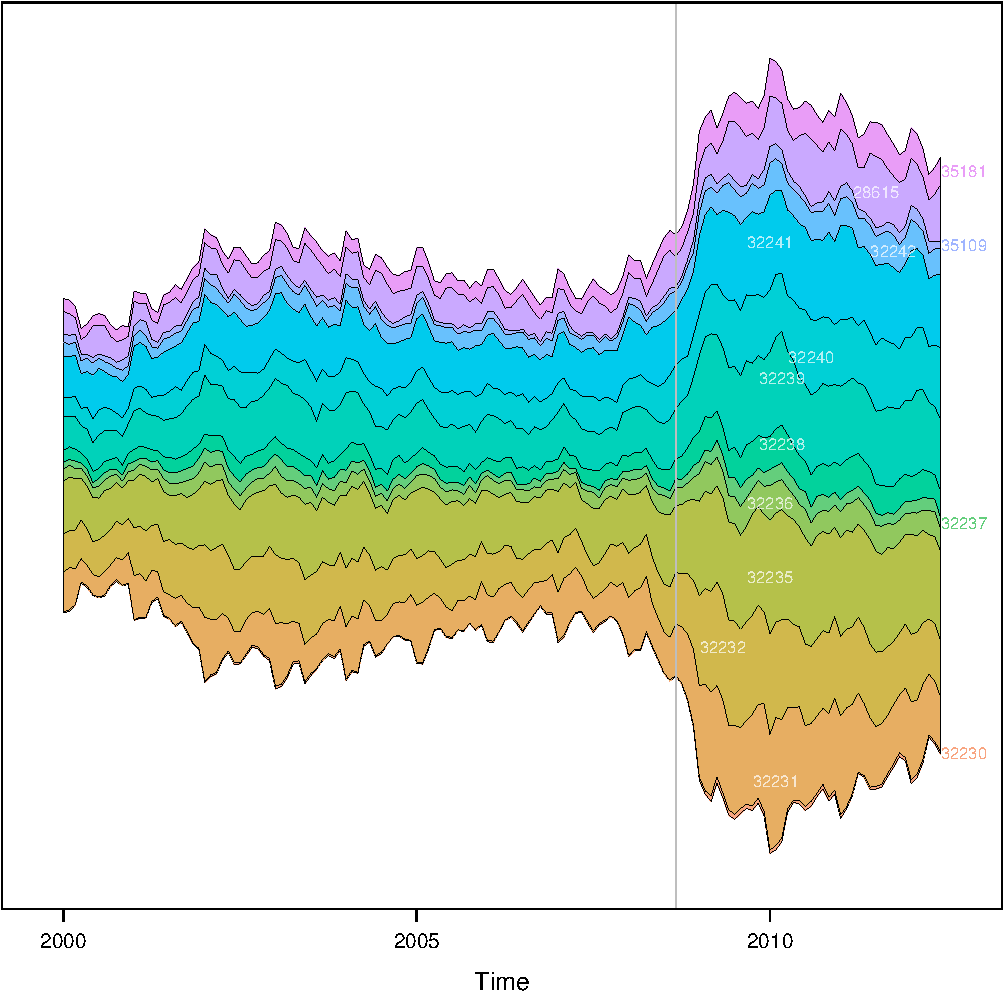
\includegraphics[width=.9\linewidth]{figs/unemployUSAThemeRiver.pdf}
\caption{ThemeRiver of unemployment in the United States. \label{fig:unemployUSAThemeRiver}}
\end{figure}

This figure can help answer several questions. For example:
\begin{itemize}
\item What is the industry or class of worker with the lowest/highest
unemployment figures during this time period?
\item What is the industry or class of worker with the lowest/highest
unemployment increases due to the financial crisis?
\item There are a number of local maxima and minima of the total
unemployment numbers. Are all the classes contributing to the
maxima/minima?  Do all the classes exhibit the same fluctuation
behavior as the global evolution?
\end{itemize}
More questions and answers can be found in the ``Current Employment
Statistics'' reports from the Bureau of Labor Statistics\footnote{The March 2012 highlights report is available at \url{http://www.bls.gov/ces/highlights032012.pdf}.}.



\subsection{\floweroneleft Panel and Prepanel Functions to Implement the ThemeRiver with \texttt{xyplot} \label{sec:themeRiverPanel}}
\label{sec:orgedc09c2}
The \texttt{xyplot} function displays information according to the class
of its first argument (methods) and to the \texttt{panel} function. We
will use the \texttt{xyplot.zoo} method (equivalent to the \texttt{xyplot.ts}
method) with a new custom \texttt{panel} function.  This new panel
function has four main arguments, three of them calculated by
\texttt{xyplot} (\texttt{x}, \texttt{y} and \texttt{groups}) and a new one, \texttt{origin}. Of
course, it includes the \texttt{...} argument to provide additional
arguments.

The first step is to create a \texttt{data.frame} with coordinates and with
the \texttt{groups} factor. The value and number of the levels will be used
in the main step of this \texttt{panel} function. With this \texttt{data.frame} we
have to calculate the \texttt{y} and \texttt{x} coordinates for each group to get a
stacked set of polygons.

This \texttt{data.frame} is in the \emph{long} format, with a row for each
observation, and where the \texttt{group} column identifies the
variable. Thus, it must be transformed to the \emph{wide} format, with a
column for each variable. With the \texttt{unstack} function, a new
\texttt{data.frame} is produced whose columns are defined according to the
formula \texttt{y \textasciitilde{} groups} and with a row for each time position. The stack
of polygons is the result of the cumulative sum of each row
(\texttt{apply(yWide, 1, cumsum)}). The origin of this sum is defined with
the corresponding \texttt{origin} argument: with \texttt{themeRiver}, the polygons
are arranged in a symmetric way.

Each column of this matrix of cumulative sums defines the \texttt{y}
coordinate of each variable (where \texttt{origin} is now the first
variable). The polygon of each variable is between this curve
(\texttt{iCol+1}) and the one of the previous variable (\texttt{iCol}). In order to
get a closed polygon, the coordinates of the inferior limit are in
reverse order. This new \texttt{data.frame} (\texttt{Y}) is in the \emph{wide} format,
but \texttt{xyplot} requires the information in the \emph{long} format: the \texttt{y}
coordinates of the polygons are extracted from the \texttt{values} column of
the \emph{long} version of this \texttt{data.frame}.

The \texttt{x} coordinates are produced in an easier way. Again, \texttt{unstack}
produces a \texttt{data.frame} with a column for each variable and a row
for each time position, but now, because the \texttt{x} coordinates are the same
for the set of polygons, the corresponding vector is constructed
directly using a combination of concatenation and repetition.

Finally, the \texttt{groups} vector is produced, repeating each element of
the columns of the original \texttt{data.frame} (\texttt{dat\$groups}) twice to
account for the forward and reverse curves of the corresponding
polygon.

The final step before displaying the polygons is to acquire the
graphical settings. The information retrieved with
\texttt{trellis.par.get} is transferred to the corresponding arguments of
\texttt{panel.polygon}.

Everything is ready for constructing the polygons. With a \texttt{for} loop,
the coordinates of the corresponding group are extracted from the \texttt{x}
and \texttt{y} vectors, and a polygon is displayed with \texttt{panel.polygon}. The
labels of each polygon (the \texttt{levels} of the original \texttt{groups}
variable, \texttt{groupLevels}) are printed inside the polygon if there is
enough room for the text (\texttt{hChar>1}) or at the right if the polygon is
too small, or if it is the first or last variable of the set. Both the
polygons and the labels share the same color (\texttt{col[i]}).

\index{Panel function}
\index{superpose.polygon@\texttt{superpose.polygon}}
\index{trellis.par.get@\texttt{trellis.par.get}}
\index{apply@\texttt{apply}}
\index{sapply@\texttt{sapply}}
\index{unstack@\texttt{unstack}}
\index{panel.text@\texttt{panel.text}}
\index{panel.polygon@\texttt{panel.polygon}}

\lstset{language=r,label= ,caption= ,captionpos=b,numbers=none}
\begin{lstlisting}
panel.flow <- function(x, y, groups, origin, ...)
{
    dat <- data.frame(x = x, y = y, groups = groups)
    nVars <- nlevels(groups)
    groupLevels <- levels(groups)
    
    ## From long to wide
    yWide <- unstack(dat, y~groups)
    ## Where are the maxima of each variable located? We will use
    ## them to position labels.
    idxMaxes <- apply(yWide, 2, which.max)
    
    ##Origin calculated following Havr.eHetzler.ea2002
    if (origin=='themeRiver') origin =  -1/2*rowSums(yWide)
    else origin = 0 
    yWide <- cbind(origin = origin, yWide)
    ## Cumulative sums to define the polygon
    yCumSum <- t(apply(yWide, 1, cumsum))
    Y <- as.data.frame(sapply(seq_len(nVars),
                              function(iCol)c(yCumSum[,iCol+1],
                                              rev(yCumSum[,iCol]))))
    names(Y) <- levels(groups)
    ## Back to long format, since xyplot works that way
    y <- stack(Y)$values
    
    ## Similar but easier for x
    xWide <- unstack(dat, x~groups)
    x <- rep(c(xWide[,1], rev(xWide[,1])), nVars)
    ## Groups repeated twice (upper and lower limits of the polygon)
    groups <- rep(groups, each = 2)
    
    ## Graphical parameters
    superpose.polygon <- trellis.par.get("superpose.polygon")
    col = superpose.polygon$col
    border = superpose.polygon$border 
    lwd = superpose.polygon$lwd 
    
    ## Draw polygons
    for (i in seq_len(nVars)){
        xi <- x[groups==groupLevels[i]]
        yi <- y[groups==groupLevels[i]]
        panel.polygon(xi, yi, border = border,
                      lwd = lwd, col = col[i])
    }
    
    ## Print labels
    for (i in seq_len(nVars)){
        xi <- x[groups==groupLevels[i]]
        yi <- y[groups==groupLevels[i]]
        N <- length(xi)/2
        ## Height available for the label
        h <- unit(yi[idxMaxes[i]], 'native') -
            unit(yi[idxMaxes[i] + 2*(N-idxMaxes[i]) +1], 'native')
        ##...converted to "char" units
        hChar <- convertHeight(h, 'char', TRUE)
        ## If there is enough space and we are not at the first or
        ## last variable, then the label is printed inside the polygon.
        if((hChar >= 1) && !(i %in% c(1, nVars))){
            grid.text(groupLevels[i],
                      xi[idxMaxes[i]],
                      (yi[idxMaxes[i]] +
                       yi[idxMaxes[i] + 2*(N-idxMaxes[i]) +1])/2,
                      gp = gpar(col = 'white', alpha = 0.7, cex = 0.7),
                      default.units = 'native')
        } else {
            ## Elsewhere, the label is printed outside
            
            grid.text(groupLevels[i],
                      xi[N],
                      (yi[N] + yi[N+1])/2,
                      gp = gpar(col = col[i], cex = 0.7),
                      just = 'left', default.units = 'native')
        }          
    }
}
  
\end{lstlisting}

With this panel function, \texttt{xyplot} displays a set of stacked
polygons corresponding to the multivariate time series (Figure
\ref{fig:themeRiverError}). However, the graphical window is not
large enough, and part of the polygons fall out of it. Why?

\lstset{language=r,label= ,caption= ,captionpos=b,numbers=none}
\begin{lstlisting}
xyplot(unemployUSA, superpose = TRUE, auto.key = FALSE,
       panel = panel.flow, origin = 'themeRiver',
       par.settings = myTheme, cex = 0.4, offset = 0,
       scales = list(y = list(draw = FALSE)))
\end{lstlisting}

\begin{figure}[htbp]
\centering
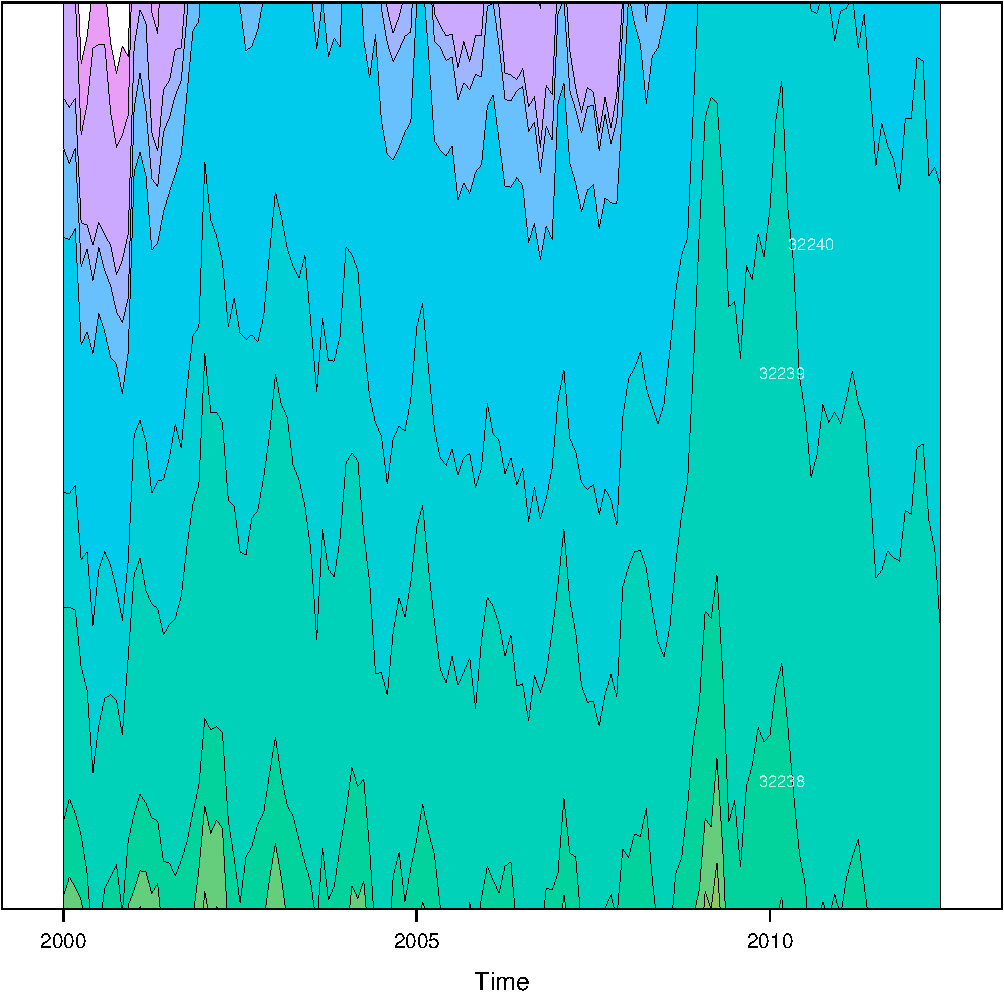
\includegraphics[height=0.45\textheight]{figs/ThemeRiverError.pdf}
\caption{First attempt of ThemeRiver. \label{fig:themeRiverError}}
\end{figure}

The problem is that \texttt{lattice} makes a preliminary estimate of the
window size using a default \texttt{prepanel} function that is unaware of the
internal calculations of our new \texttt{panel.flow} function. The solution
is to define a new \texttt{prepanel.flow} function. 

The input arguments and first lines are the same as in
\texttt{panel.flow}. The output is a list whose elements are the limits for
each axis (\texttt{xlim} and \texttt{ylim}), and the sequence of differences (\texttt{dx}
and \texttt{dy}) that can be used for the aspect and banking
calculations. 

The limits of the x-axis are defined with the range of the time index,
while the limits of the y-axis are calculated with the minimum of the
first column of \texttt{yCumSum} (the origin line) and with the maximum of
its last column (the upper line of the cumulative sum).

\lstset{language=r,label= ,caption= ,captionpos=b,numbers=none}
\begin{lstlisting}
prepanel.flow <- function(x, y, groups, origin,...)
{
    dat <- data.frame(x = x, y = y, groups = groups)
    nVars <- nlevels(groups)
    groupLevels <- levels(groups)
    yWide <- unstack(dat, y~groups)
    if (origin=='themeRiver') origin =  -1/2*rowSums(yWide)
    else origin = 0
    yWide <- cbind(origin = origin, yWide)
    yCumSum <- t(apply(yWide, 1, cumsum))
    
    list(xlim = range(x),
         ylim = c(min(yCumSum[,1]), max(yCumSum[,nVars+1])),
         dx = diff(x),
         dy = diff(c(yCumSum[,-1])))
}
\end{lstlisting}


\section{Interactive graphics \label{sec:interactive_horizontal}}
\label{sec:org1d734a3}
This section describes the interactive alternatives of the static
figures included in the previous sections with several packages:
\texttt{dygraphs}, \texttt{highcharter}, \texttt{plotly}, \texttt{streamgraph}, and \texttt{gridSVG}.

\texttt{dygraphs}, \texttt{highcharter}, \texttt{plotly}, and \texttt{streamgraph} are \texttt{R} interfaces to
JavaScript libraries based on the \texttt{htmlwidgets} package, while the
\texttt{gridSVG} package converts a \texttt{grid} graphic object into an SVG file.

\subsection{Dygraphs \label{sec:dygraphs}}
\label{sec:org3cef033}
The \texttt{dygraphs} package is an interface to the \texttt{dygraphs} JavaScript
library, and provides facilities for charting time-series. It works
automatically with \texttt{xts} time series objects, or with objects than can
be coerced to this class. The result is an interactive graph, where
values are displayed according to the mouse position over the time
series. Regions can be selected to zoom into a time period. The figure
\ref{fig:dygraphs} is an snapshot of the interactive graph.

\index{Packages!dygraphs@\texttt{dygraphs}}

\lstset{language=r,label= ,caption= ,captionpos=b,numbers=none}
\begin{lstlisting}
library(dygraphs)

dyTemp <- dygraph(aranjuez[, c("TempMin", "TempAvg", "TempMax")],
                  main = "Temperature in Aranjuez",
                  ylab = "ºC")

dyTemp
\end{lstlisting}

\begin{figure}[htbp]
\centering
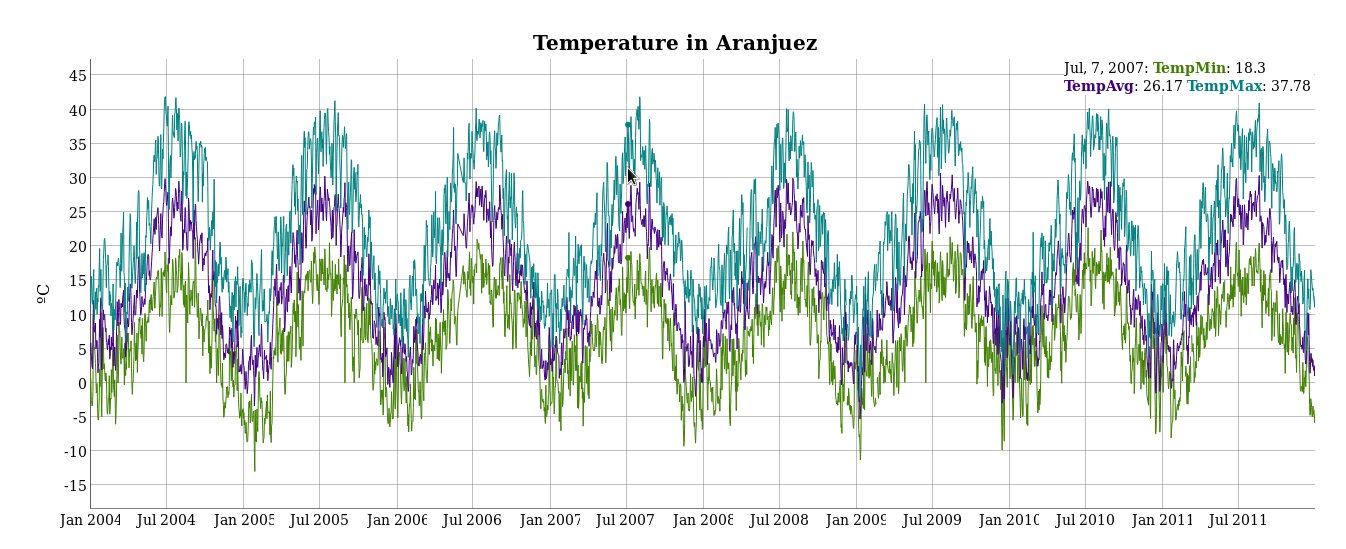
\includegraphics[width=.9\linewidth]{figs/dygraphs_aranjuez.png}
\caption{Snapshot of an interactive graphic produced with \texttt{dygraphs}. \label{fig:dygraphs}}
\end{figure}



You can customize \texttt{dygraphs} by piping additional commands onto the original graphic.  The function \texttt{dyOptions} provides several choices for the graphic, and the function \texttt{dyHighlight} configures options for data series mouse-over highlighting. For example, with the next code the semi-transparency value of the non-selected lines is reduced and the width of selected line is increased (Figure \ref{fig:dygraphs_selected}).

\lstset{language=r,label= ,caption= ,captionpos=b,numbers=none}
\begin{lstlisting}
dyTemp %>%
    dyHighlight(highlightSeriesBackgroundAlpha = 0.2,
                highlightSeriesOpts = list(strokeWidth = 2))
\end{lstlisting}

\begin{figure}[htbp]
\centering
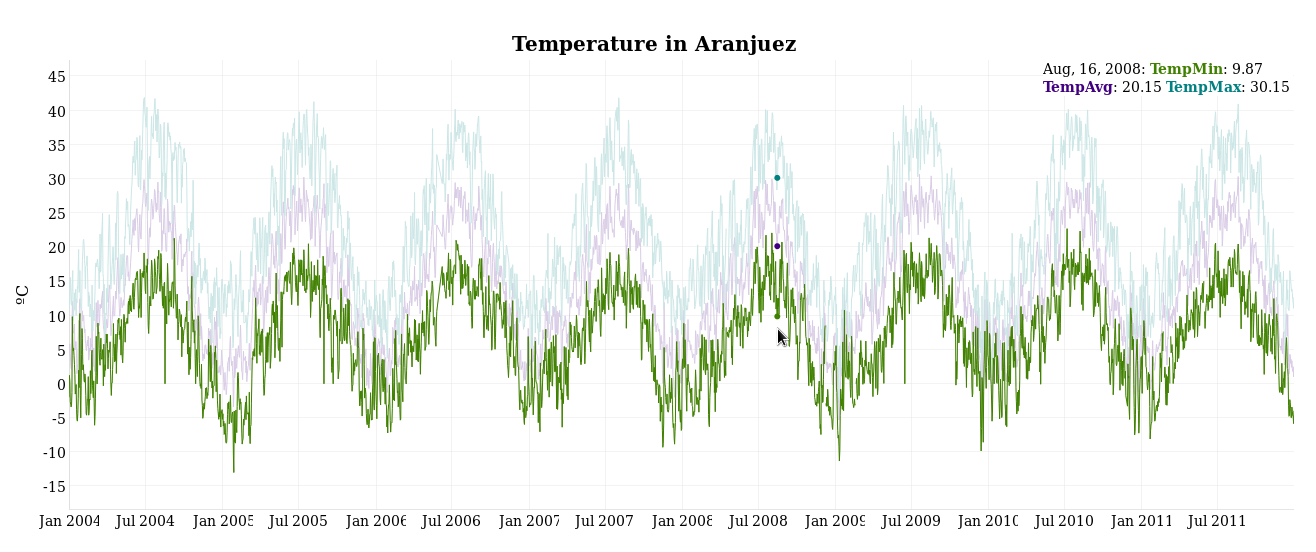
\includegraphics[width=.9\linewidth]{figs/dygraphs_aranjuez_selected.png}
\caption{Snapshot of a selection in an interactive graphic produced with \texttt{dygraphs}. \label{fig:dygraphs_selected}}
\end{figure}

An alternative approach to depict the upper and lower variables of this time series is with a shaded region. The \texttt{dySeries} function accepts a character vector of length 3 that specifies a set of input column names to use as the lower, value, and upper for a series with a shaded region  around it (Figure \ref{fig:dygraphs_maxmin}).
\lstset{language=r,label= ,caption= ,captionpos=b,numbers=none}
\begin{lstlisting}
dygraph(aranjuez[, c("TempMin", "TempAvg", "TempMax")],
        main = "Temperature in Aranjuez",
        ylab = "ºC") %>%
    dySeries(c("TempMin", "TempAvg", "TempMax"),
             label = "Temperature")
\end{lstlisting}

\begin{figure}[htbp]
\centering
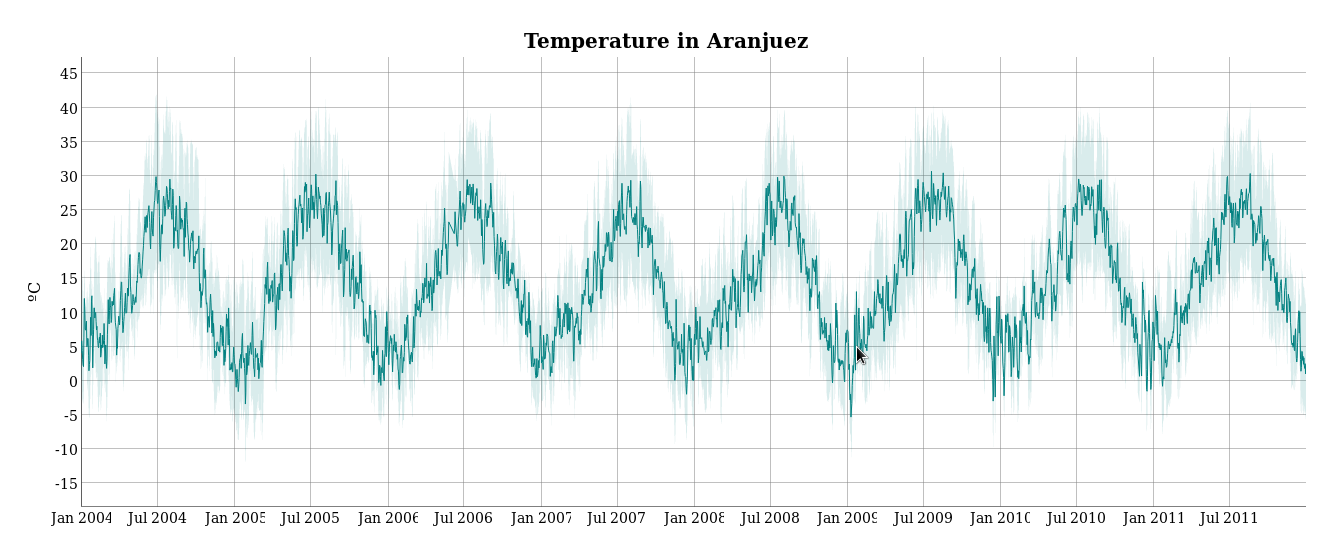
\includegraphics[width=.9\linewidth]{figs/dygraphs_aranjuez_maxmin.png}
\caption{Shaded region between upper and lower values around a time series. \label{fig:dygraphs_maxmin}}
\end{figure}

\subsection{Highcharter \label{sec:highcharter}}
\label{sec:org3cdb71b}

The \texttt{highcharter} package is an interface to the \texttt{highcharts}
JavaScript library, with a wide spectrum of graphics
solutions. Displaying time series with this package can be achieved
with the combination of the generic \texttt{highchart} function and several
calls to the \texttt{hc\_add\_series\_xts} function through the pipe \texttt{\%>\%}
operator.  Once again, the result is an interactive graph with
selection and zoom capabilities. Figure \ref{fig:highcharter} is an
snapshot of the interactive graph, and Figure
\ref{fig:highcharter_zoom} is an snapshot of this same graph with
zoom.

\index{Packages!highcharter@\texttt{highcharter}}

\lstset{language=r,label= ,caption= ,captionpos=b,numbers=none}
\begin{lstlisting}
library(highcharter)
library(xts)

aranjuezXTS <- as.xts(aranjuez)

highchart() %>%
    hc_add_series_xts(name = 'TempMax',
                      aranjuezXTS[, "TempMax"]) %>%
    hc_add_series_xts(name = 'TempMin',
                      aranjuezXTS[, "TempMin"]) %>%
    hc_add_series_xts(name = 'TempAvg',
                      aranjuezXTS[, "TempAvg"])

\end{lstlisting}

\begin{figure}[htbp]
\centering
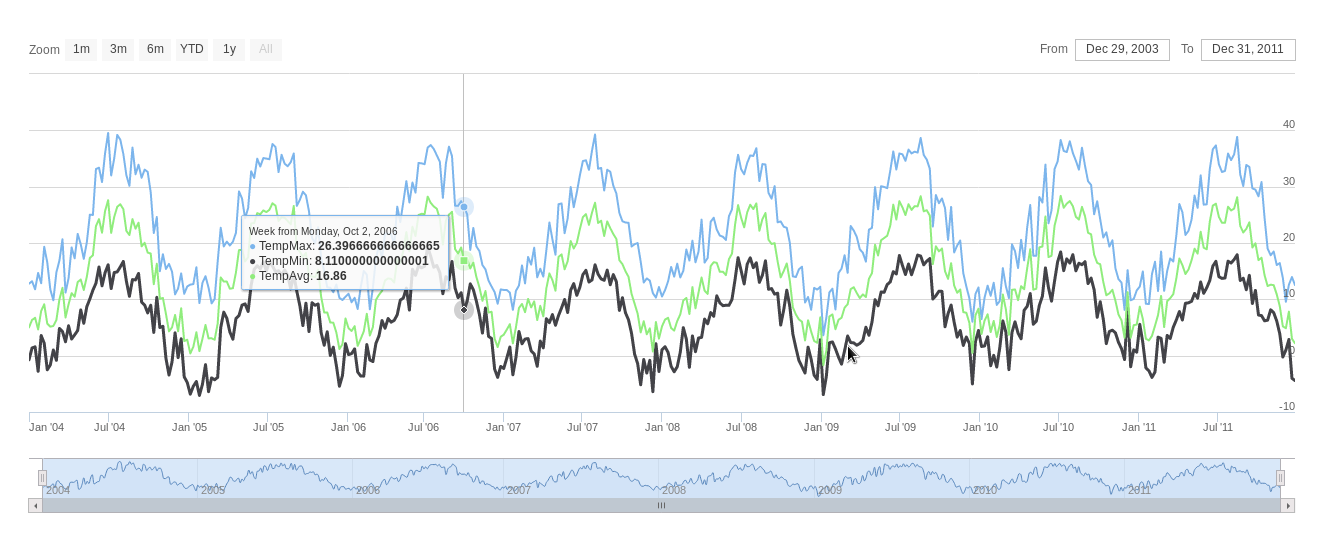
\includegraphics[width=.9\linewidth]{figs/highcharter_aranjuez.png}
\caption{Snapshot of an interactive graphic produced with \texttt{highcharter}. \label{fig:highcharter}}
\end{figure}

\begin{figure}[htbp]
\centering
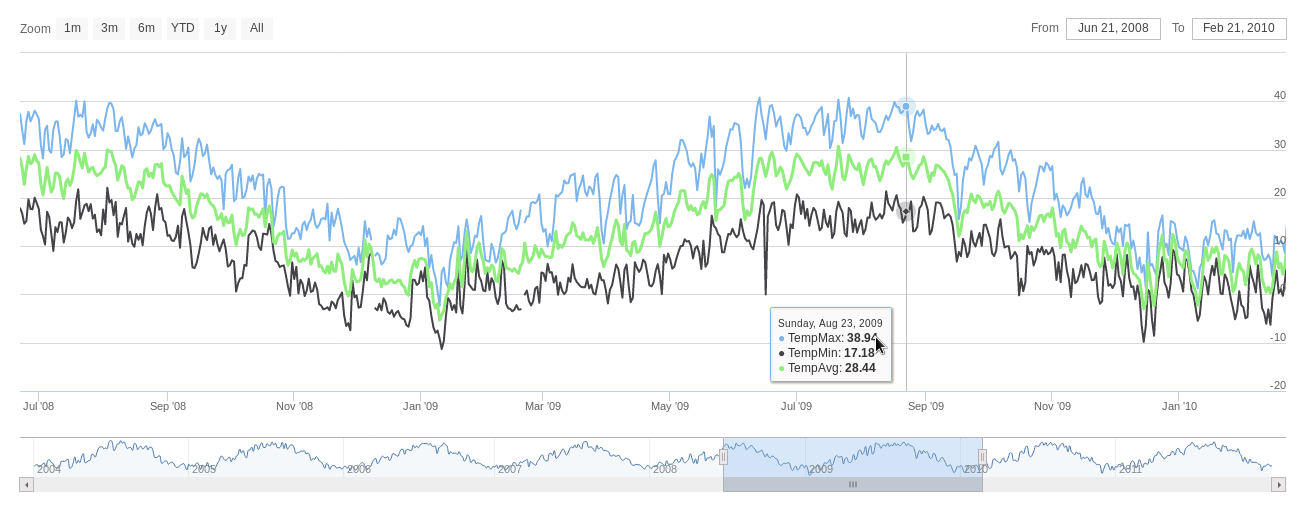
\includegraphics[width=.9\linewidth]{figs/highcharter_aranjuez_zoom.png}
\caption{Snapshot of a zoom in an interactive graphic produced with \texttt{highcharter}. \label{fig:highcharter_zoom}}
\end{figure}



\subsection{plotly \label{sec:plotly_horizontal}}
\label{sec:orgc0e930f}

The \texttt{plotly} package is an interface to the \texttt{plotly} JavaScript
library, also with a wide spectrum of graphics solutions. This package
does not provide any function specifically focused on time
series. Thus, the time series object has to be transformed in a
\texttt{data.frame} including a column for the time index. If the
\texttt{data.frame} is in \emph{wide} format (one column per variable), each
variable will be represented with a call to the \texttt{add\_lines}
function. However, if the \texttt{data.frame} is in \emph{long} format (a column
for values, and a column for variable names) only one call to
\texttt{add\_lines} is required. The next code follows this approach using the
combination of \texttt{fortify}, to convert the \texttt{zoo} object into a
\texttt{data.frame}, and \texttt{melt}, to transform from wide to long format.

\index{fortify@\texttt{fortify}}
\index{melt\texttt{melt}}

\lstset{language=r,label= ,caption= ,captionpos=b,numbers=none}
\begin{lstlisting}
aranjuezDF <- fortify(aranjuez[,
                               c("TempMax",
                                 "TempAvg",
                                 "TempMin")],
                      melt = TRUE)

summary(aranjuezDF)
\end{lstlisting}

\begin{verbatim}
    Index                Series         Value        
Min.   :2004-01-01   TempMax:2898   Min.   :-12.980  
1st Qu.:2005-12-29   TempAvg:2898   1st Qu.:  7.107  
Median :2008-01-09   TempMin:2898   Median : 13.560  
Mean   :2008-01-03                  Mean   : 14.617  
3rd Qu.:2010-01-03                  3rd Qu.: 21.670  
Max.   :2011-12-31                  Max.   : 41.910  
                                    NA's   :10
\end{verbatim}


Figure \ref{fig:plotly} is a snapshot of the interactive graphic produce
with the generic function \texttt{plot\_ly} connected with \texttt{add\_lines} through
the pipe operator, \texttt{\%>\%}.

\index{Packages!plotly@\texttt{plotly}}

\lstset{language=r,label= ,caption= ,captionpos=b,numbers=none}
\begin{lstlisting}
library(plotly)

plot_ly(aranjuezDF) %>%
    add_lines(x = ~ Index,
              y = ~ Value,
              color = ~ Series)

\end{lstlisting}

\begin{figure}[htbp]
\centering
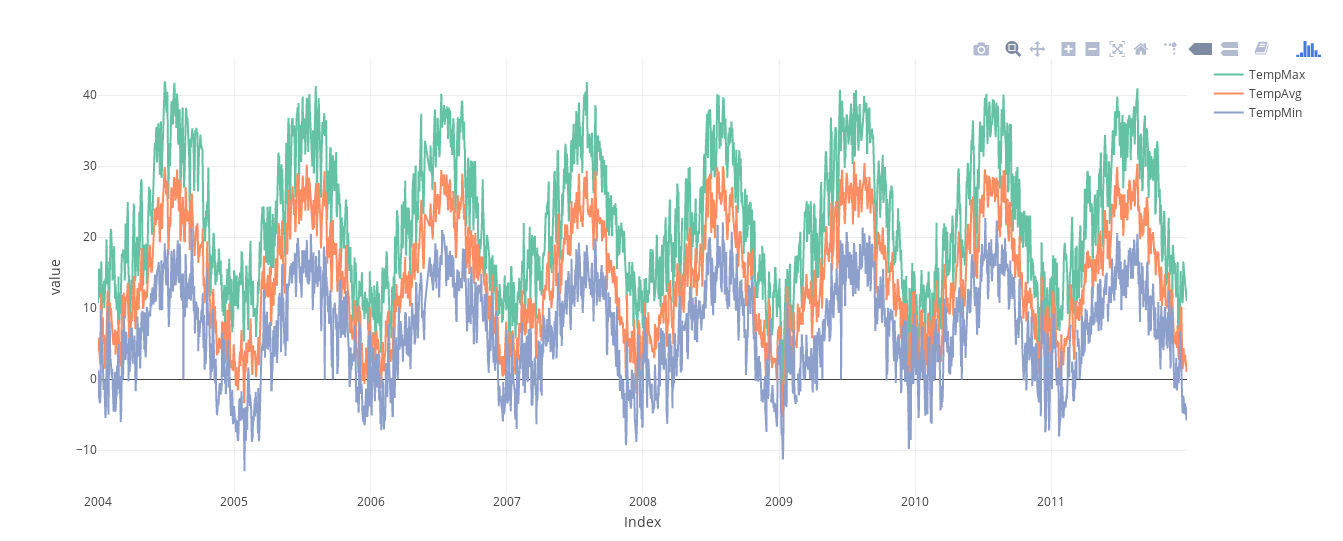
\includegraphics[width=.9\linewidth]{figs/plotly_aranjuez.png}
\caption{Snapshot of an interactive graphic produced with \texttt{plotly}. \label{fig:plotly}}
\end{figure}

\begin{figure}[htbp]
\centering
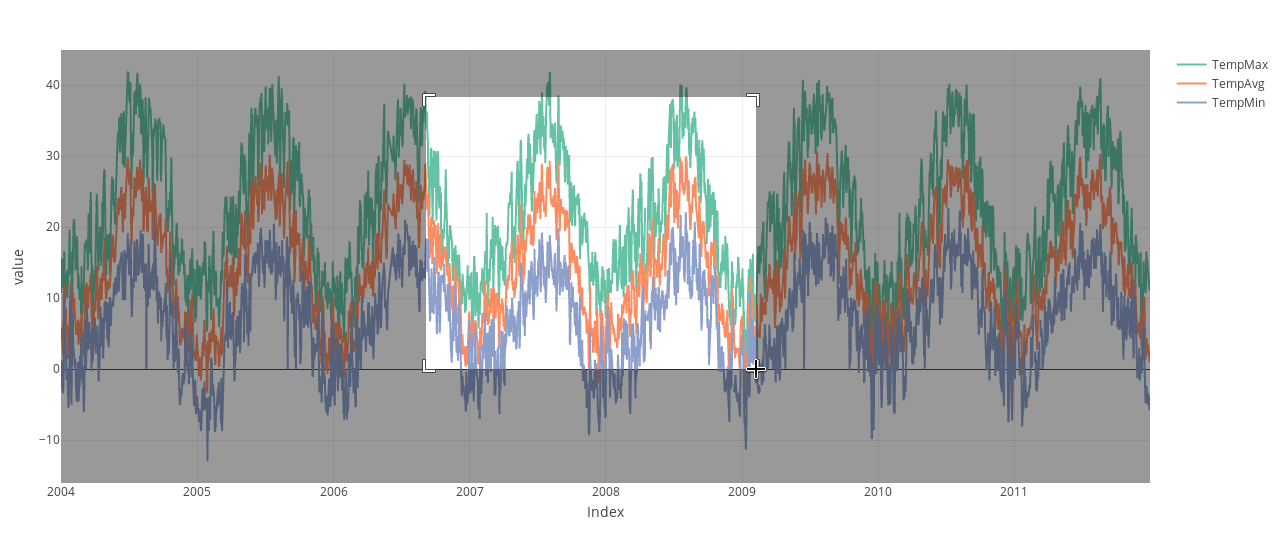
\includegraphics[width=.9\linewidth]{figs/plotly_aranjuez_zoom.png}
\caption{Snapshot of a zoom in an interactive graphic produced with \texttt{plotly}. \label{fig:plotly_zoom}}
\end{figure}


\subsection{\floweroneleft Interaction with \texttt{gridSVG}}
\label{sec:orgdeafeb5}
The \texttt{gridSVG} package provides functions to convert \texttt{grid}-based \texttt{R}
graphics to an SVG format. It provides several functions to add
dynamic and interactive capabilities to \texttt{R} graphics. In this section
we will use \texttt{grid.script}, a function to add JavaScript code to a
plot.

The first step is to specify which component of the scene
will run the JavaScript code. The \texttt{grid.ls} function  returns a
listing of the names of grobs or viewports included in the graphic
output: only the lines will be connected with the JavaScript
code. 

\index{Packages!gridSVG@\texttt{gridSVG}}
\index{grid.ls@\texttt{grid.ls}}

\lstset{language=r,label= ,caption= ,captionpos=b,numbers=none}
\begin{lstlisting}
library(gridSVG)
## grobs in the graphical output
pNavarra
grobs <- grid.ls(print = FALSE)
## only interested in some of them
nms <- grobs$name[grobs$type == "grobListing"]
idxNames <- grep('lines', nms)
IDs <- nms[idxNames]
\end{lstlisting}

The second step is to modify each \texttt{grob} (graphical object) to add
attributes that specify when it will call JavaScript code. For each
line identified with the elements of the \texttt{IDs} vector and associated
to a meteorological station, the \texttt{navarra} object is accessed to
extract the annual mean value of the daily radiation and the
abbreviated name of the corresponding station (\texttt{info}).  The
\texttt{grid.garnish} function adds attributes to the \texttt{grob} of each line so
that when the mouse moves over a \texttt{grob}, the line is highlighted and
colored in red (\texttt{highlight}). When the mouse hovers out of the \texttt{grob},
the \texttt{hide} function sets back the default values of line width and
transparency, but uses the green color to denote that this line has
been already visited. In addition, because the browsers display the
content of the title attribute with a default tooltip, \texttt{grid.garnish}
sets this attribute to \texttt{info}.

\index{grid.garnish@\texttt{grid.garnish}}

\lstset{language=r,label= ,caption= ,captionpos=b,numbers=none}
\begin{lstlisting}
for (id in unique(IDs))
{
    ## extract information from the data
    ## according to the ID value
    i <- strsplit(id, '\\.')
    i <- sapply(i, function(x)as.numeric(x[5]))
    ## Information to be attached to each line: annual mean of daily
    ## radiation and abbreviated name of the station
    dat <- round(mean(navarra[,i], na.rm = TRUE), 2)
    info <- paste(names(navarra)[i], paste(dat, collapse = ','),
                  sep = ': ')
    ## attach SVG attributes
    grid.garnish(id,
                 onmouseover = "highlight(evt)",
                 onmouseout = "hide(evt)",
                 title = info)
}
\end{lstlisting}

These JavaScript functions are included in a script file named
\texttt{highlight.js} (available at the website of the book). It can be
added as an additional object with \texttt{grid.script}.

\index{grid.script@\texttt{grid.script}}

\lstset{language=r,label= ,caption= ,captionpos=b,numbers=none}
\begin{lstlisting}
grid.script(filename="highlight.js")
\end{lstlisting}

This script is easy to understand, even without previous
JavaScript knowledge:
\index{JavaScript}
\begin{verbatim}
highlight = function(evt){',
      evt.target.setAttribute('opacity', '1');
      evt.target.setAttribute('stroke', 'red');
      evt.target.setAttribute('stroke-width', '1');
  }
  
hide = function(evt){
      evt.target.setAttribute('opacity', '0.3');
      evt.target.setAttribute('stroke', green');
      evt.target.setAttribute('stroke-width', '0.3');
  }
\end{verbatim}

Finally, \texttt{gridToSVG} exports the whole scene to SVG. 

\index{grid.export@\texttt{grid.export}}

\lstset{language=r,label= ,caption= ,captionpos=b,numbers=none}
\begin{lstlisting}
grid.export('figs/navarraRadiation.svg')
\end{lstlisting}

A snapshot of the result, as viewed in a browser with a line
highlighted, is shown in Figure \ref{fig:navarraSVG}. Open the SVG
file with your browser, explore it using the horizon graph (Figure
\ref{fig:navarraHorizonplot}) as a reference, and try to answer the
questions raised with that graphic.

\begin{figure}[htbp]
\centering
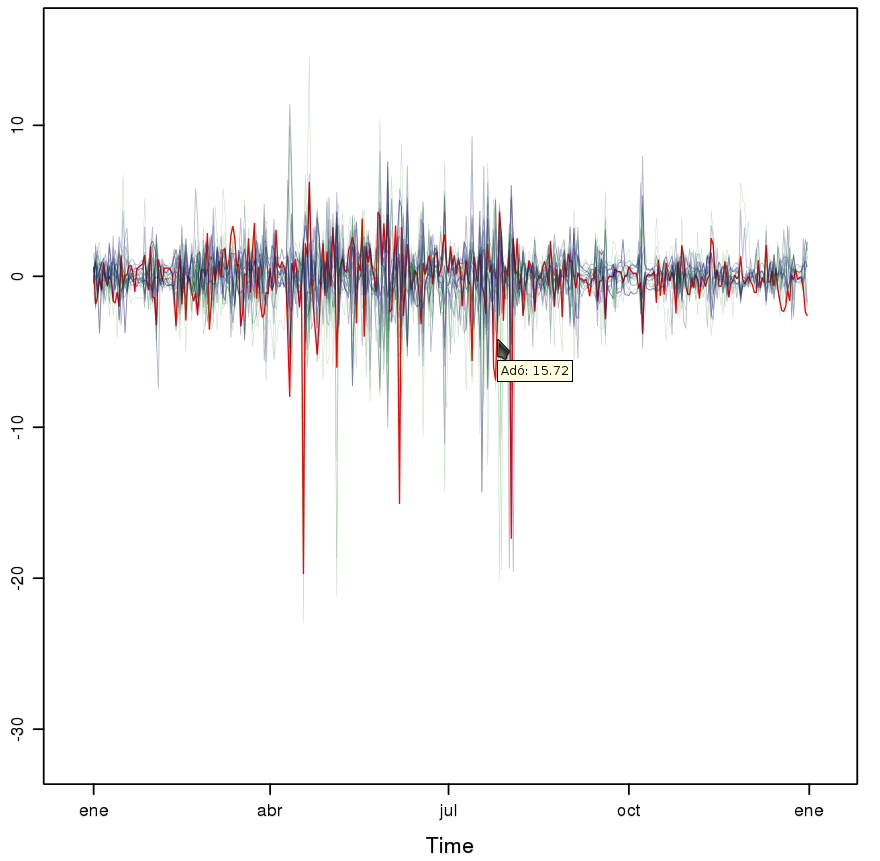
\includegraphics[width=.9\linewidth]{figs/navarraSVG_captura.png}
\caption{Snapshot of an SVG graphic produced with \texttt{gridSVG}. \label{fig:navarraSVG}}
\end{figure}


\subsection{streamgraph \label{sec:interactive_streamgraph}}
\label{sec:org7efd97d}

The \texttt{streamgraph} package\footnote{The \texttt{streamgraph} package, \url{http://hrbrmstr.github.io/streamgraph/}, is not available in CRAN. It can be installed using the \texttt{devtools} or the \texttt{remotes} package.} creates interactive stream graphs based on
the \texttt{htmlwidgets} package and the \texttt{D3.js} JavaScript library. Its main
function, \texttt{streamgraph}, requires a \texttt{data.frame} as the first
argument. Besides, its three next arguments, \texttt{key}, \texttt{value}, and
\texttt{date}, makes this function a good candidate to work together with
\texttt{fortify} and \texttt{melt}.

\index{fortify@\texttt{fortify}}
\index{melt\texttt{melt}}

\lstset{language=r,label= ,caption= ,captionpos=b,numbers=none}
\begin{lstlisting}
unemployDF <- fortify(unemployUSA, melt = TRUE)

head(unemployDF)
\end{lstlisting}

\begin{verbatim}
     Index Series Value
1 ene 2000  32230    19
2 feb 2000  32230    25
3 mar 2000  32230    17
4 abr 2000  32230    20
5 may 2000  32230    27
6 jun 2000  32230    13
\end{verbatim}

Figures \ref{fig:streamgraph_interactive} and
\ref{fig:streamgraph_interactive_selected} are snapshots of the
interactive graphic created with the functions \texttt{streamgraph},
\texttt{sg\_axis}, and \texttt{sg\_fill\_brewer}, connected through the pipe operator,
\texttt{\%>\%}.

\index{Packages!streamgraph\texttt{streamgraph}}

\lstset{language=r,label= ,caption= ,captionpos=b,numbers=none}
\begin{lstlisting}
## remotes::install_github("hrbrmstr/streamgraph")
library(streamgraph)
\end{lstlisting}

\lstset{language=r,label= ,caption= ,captionpos=b,numbers=none}
\begin{lstlisting}
streamgraph(unemployDF,
            key = "Series",
            value = "Value",
            date = "Index") %>%
    sg_axis_x(1, "year", "%Y") %>%
    sg_fill_brewer("Set1")
\end{lstlisting}

\begin{figure}[htbp]
\centering
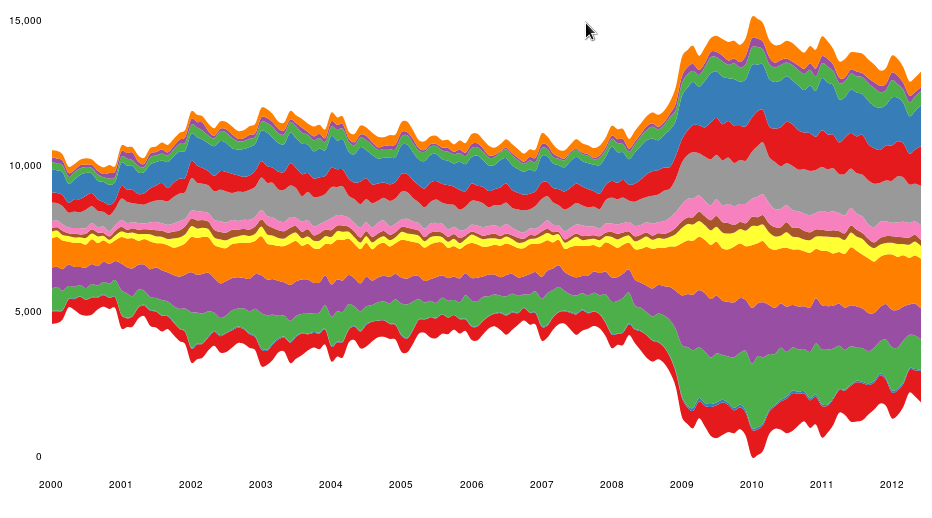
\includegraphics[width=.9\linewidth]{figs/streamgraph_interactive.png}
\caption{Streamgraph created with the \texttt{streamgraph} package, without selection. \label{fig:streamgraph_interactive}}
\end{figure}

\begin{figure}[htbp]
\centering
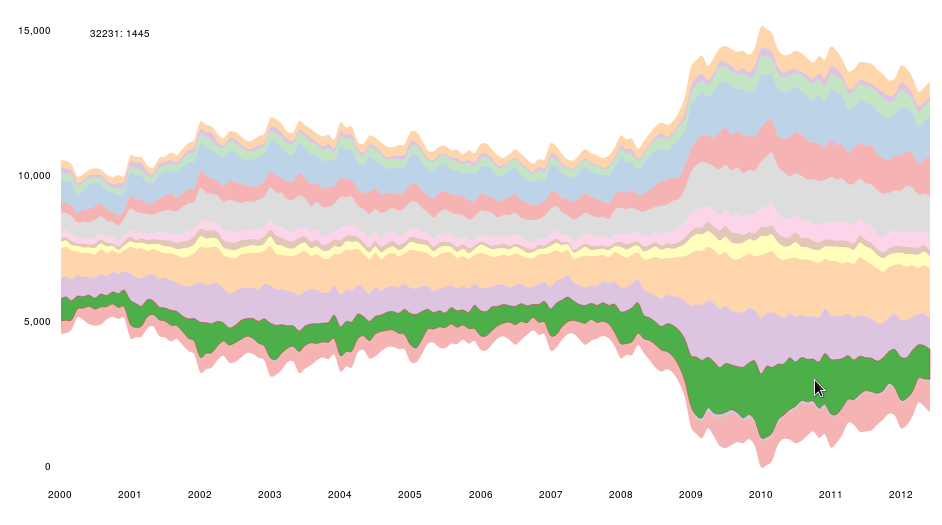
\includegraphics[width=.9\linewidth]{figs/streamgraph_interactive_selected.png}
\caption{Streamgraph created with the \texttt{streamgraph} package, with a selection. \label{fig:streamgraph_interactive_selected}}
\end{figure}
